\documentclass[a4paper]{report}

% \usepackage[utf8]{inputenc}
% \usepackage[T1]{fontenc}
% \usepackage{textcomp}
\usepackage[english]{babel}
\usepackage{amsmath, amssymb}
\usepackage[separate-uncertainty=true, multi-part-units=single]{siunitx}
\usepackage[]{subfig}
\usepackage[colorlinks=true, anchorcolor=blue, linkcolor=blue, citecolor=blue, bookmarks=false,hyperfootnotes=false]{hyperref}
\usepackage[margin=1in]{geometry}
\usepackage{color,soul}
\usepackage{tabularx}

% figure support
\usepackage{import}
\usepackage{xifthen}
\pdfminorversion=7
\usepackage{pdfpages}
\usepackage{transparent}
\usepackage{physics}
\graphicspath{ {./figures/} }
% \setlength{\parindent}{0pt}
\usepackage{chngcntr}
\usepackage{verbatim}
\usepackage{indentfirst}
\numberwithin{equation}{section}
\counterwithin{figure}{section}
\newcommand{\incfig}[1]{%
		\def\svgwidth{\columnwidth}
		\import{./figures/}{#1.pdf_tex}

}

\pdfsuppresswarningpagegroup=1

% for citations / references
\usepackage[style=ieee]{biblatex}
\addbibresource{cavities-report.bib}

\begin{document}

%----------------------------------------------------------------------------------------
%	TITLE PAGE
%----------------------------------------------------------------------------------------
\begin{titlepage} % Suppresses displaying the page number on the title page and the subsequent page counts as page 1
	\newcommand{\HRule}{\rule{\linewidth}{0.5mm}} % Defines a new command for horizontal lines, change thickness here
	
	\center % Centre everything on the page
	%------------------------------------------------
	%	Headings
	%------------------------------------------------
	
	\textsc{\LARGE Rheinische Friedrich-Wilhelms-Universit\"at Bonn }\\[4cm] % Main heading such as the name of your university/college
	
	\textsc{\Large Advanced Laboratory Course}\\[0.5cm] % Major heading such as course name
	
	\textsc{\large Performed on: March 16, 2022}\\[0.5cm] % Minor heading such as course title
	
	%------------------------------------------------
	%	Title
	%------------------------------------------------
	
	\HRule\\[0.4cm]
	
	{\huge\bfseries E106: Cavities}\\[0.4cm] % Title of your document
	
	\HRule\\[1.5cm]
	
	%------------------------------------------------
	%	Author(s)
	%------------------------------------------------
	
	\begin{minipage}{0.4\textwidth}
		\begin{flushleft}
			\large
			\textit{Authors}\\
			Paarth Thakkar \\
			Keito Watanabe
		\end{flushleft}
	\end{minipage}
	~
	\begin{minipage}{0.4\textwidth}
		\begin{flushright}
			\large
			\textit{Head Tutor}\\
			Dr. Michael Switka
		\end{flushright}
	\end{minipage}
	
	% If you don't want a supervisor, uncomment the two lines below and comment the code above
	%{\large\textit{Author}}\\
	%John \textsc{Smith} % Your name
	
	%------------------------------------------------
	%	Date
	%------------------------------------------------
	
	%\vfill\vfill\vfill % Position the date 3/4 down the remaining page
	\vfill\vfill
	
	%{\large\today} % Date, change the \today to a set date if you want to be precise
	
	%------------------------------------------------
	%	Logo
	%------------------------------------------------
	
	%\vfill\vfill
	%\includegraphics[width=0.2\textwidth]{placeholder.jpg}\\[1cm] % Include a department/university logo - this will require the graphicx package
	 
	%----------------------------------------------------------------------------------------
	
	\vfill % Push the date up 1/4 of the remaining page
	
\end{titlepage}

\tableofcontents

\chapter{Introduction}
In this experiment, we study the various characteristics of a cavity. These characteristics help quantify how good the cavity is. Before talking about cavities themselves though, it is important to understand why we are studying them. Cavity resonators are important optical and microwave system components \cite{Weng}. The main principle is that it has constructive and destructive interference pattern inside and enclosed region. They can be used as a filters, or as antennas or in lasers. They also have a wide range of application in particle accelerators \cite{accelerator}. \\
x
In today's report, we will first discuss the theoretical background, which gives us an insight on the working of cavities and how it works. Then we move on to the experimental setup and procedure. We end with results from our analysis and discussion. 

\chapter{Theoretical Background}

\section{Waveguides}
In order to understand cavities, we start off with the discussion on waveguides.
An electromagnetic wave, when confined to the interior of a hollow pipe is
called a waveguide. We shall closely follow the laboratory script \cite{Hillert} for our report.The
generalized Maxwell equations in terms of E-field and H-field are given by:

\begin{align}
		\curl {\vb{{E}}} &= - \pdv{{B}}{t} \\
		\div{\vb{D}} &= \rho \\
		\curl {\vb{{H}}} &= \vec{j} + \pdv{{D}}{t} \\
		\div{\vb{{B}}} &= 0 
\end{align}

In vacuum, these equations become: 
\begin{align}
		\curl {\vb{{E}}} &= \mu_0 \cdot \pdv{{H}}{t} \\ 
		\div{\vb{{E}}} &= 0 \\
		\curl {\vb{{H}}} &= \epsilon_{0} \cdot \pdv{{E}}{t} \\
		\div{\vb{{H}}} &= 0
\end{align}

Upon solving these equations, we get plane wave solutions which looks like this: 
\begin{align*}
		\Delta \vec{E}\left(\vec{r}\right) + \frac{\omega}{c^2} \vec{E}\left(\vec{r}\right) = 0 \\
		\Delta \vec{B}\left(\vec{r}\right) + \frac{\omega}{c^2} \vec{B}\left(\vec{r}\right) = 0 
\end{align*}

Now, let us look at a waveguide which is aligned along the z-direction. Taking
the ansatz $\vec{E} = \vec{E}(x,y).e^{i(\omega t -kz)}$ and the separation
$\Delta = \Delta_{\perp} + \pdv[2]{}{z}$, for the longitudinal fields yields: 

\begin{align}
		\Delta_{\perp}E_{z} + k_{c}^2 E_{z} = 0 \\
		\Delta_{\perp}H_{z} + k_{c}^2 H_{z} = 0 
\end{align}
where 
\[
		k_{c}^2 = \frac{\omega^2 }{c^2 } - k^2   
\]
The quantity $k_{c} $ is called the critical wave number and is a characteristic
property of the cavity, as we shall see. Solving these equations further, we see
that it is sufficient to know the longitudinal fields, $E_{z} $ and $B_{z} $
because we can easily determine the transverse components from them. 
\begin{align} 
		ik_{c}^2 \vec{E}_{\perp} = k \vec{\nabla}_{\perp}E_{z} + \omega \mu _{0} \vec{\nabla}_{\perp}H_{z} \times \hat{e}_{z} \label{trans1} \\
		ik_{c}^2 \vec{H}_{\perp} = k \vec{\nabla}_{\perp}H_{z} - \omega \epsilon_{0} \vec{\nabla}_{\perp} E_{z} \times \hat{e}_{z} \label{trans2}     
\end{align}

Now, there are two waves to classify these waves: 
\begin{enumerate}
		\item $k_{c}^2 = 0  $ 
				\begin{enumerate}
						\item $\vec{\Delta_{\perp} }E_{z}  \ne 0$ and
						$\vec{\Delta}_{\perp}H_{z} \ne 0  $: HE or EH hybrid
						waves.
						\item $\vec{\Delta_{\perp} }E_{z}  = 0$ and
						$\vec{\Delta}_{\perp}H_{z} = 0  $: TEM waves.
				\end{enumerate}
		\item $k_{c}^2 \ne 0  $ In this case we do not get any propagation if
		$\omega \leq c \cdot k_{c} $. These waves are called evanescent waves or
		the cut off condition. The possible propagation modes are: 
		\begin{enumerate}
				\item $E_{z}=0 $: TE (transversal electric) or H waves.
				\item $H_{z}=0 $: TM (transversal magnetic) or E waves.
		\end{enumerate}
		
\end{enumerate}

Corresponding to this critical wave, we have a critical frequency, which is
$\omega_{c}=k_{c}.c $, below which there is no propagation. One interesting
thing to note here is that for a hollow waveguide, only TE or TM modes are
possible, TEM is not, because no wave would exist in this case \cite{Griffiths}. But for
a coaxial cable, which consists of straight wire surrounded by a conduction
sheath, we can get TEM modes.

\subsection{Cylindrical waveguides}
We now consider a cylindrical waveguide with an inner radius a. This imposes the
following boundary conditions to the walls of the waveguide:
\begin{itemize}
		\item $E_{\phi} = 0$, $E_{z} = 0 $ \text{for} $r = a$ 
		\item $H_{r} = 0 $ \text{for} $r = a$ 
\end{itemize}

The field distribution solution for a cylindrical waveguide can be separated
into angular and radial parts, whose solutions are then given by the
Bessel/Neumann functions. These can be then substituted in the
eq.(\ref{trans1})-(\ref{trans2}) and upon imposing the constraints from the
boundary condition gives us the corresponding TE- and TM-modes.

\subsection{Cylindrical waveguides resonator}
The time has now come, to talk about cavities itself. If we now insert two
conducting plates perpendicular to the z-axis, the incoming wave is reflected
completely, giving us standing waves. Because of this, the z-dependence changes
like: 

\[
		a \cdot e^{ikz} \implies A \cdot \sin\left(kz + \phi_{0}\right)    
\]
The following condition is imposed so that the longitudinal boundary conditions
are fulfilled: $k = p\cdot \pi /l $. The longitudinal field looks like: 
\begin{align*}
		\mathbf{TE_{mnp}-Modes}&: H_{z} = H_{mn}\cdot J_{m} \left(k_{c}r \right) \cos\left(m \phi \right) \cdot \sin\left(p \pi / l \cdot z \right) \cdot e^{\omega_{mnp}t}; \\  &\text{ where } k_{c}a=j_{mn}^{'}  \\
		\mathbf{TM_{mnp}-Modes}&: E_{z} = E_{mn}\cdot J_{m}^{'}  \left(k_{c}r \right) \cos\left(m \phi \right) \cdot \cos\left(p \pi / l \cdot z \right) \cdot e^{\omega_{mnp}t}; \\  &\text{ where } k_{c}a=j_{mn} 
\end{align*}
For resonant frequency, we have:

\[
		\omega_{mnp} = c \cdot \sqrt{\left(j_{mn}/a\right)^2 + \left(p \pi / l\right)^2} 
\]

Here, $J_{m}$ is the $m$-th Bessel function, $J_{m}^{'} $ is its derivative. And
$j_{mn}$ and $j_{mn}^{'}$ are the $n$-th zeropoints of the $m$-th Bessel
function and its derivative.

The resonant modes can be written in the linear form as:

\begin{equation} \label{eqn:res_freq}
		\left(d \nu \right)^2 = \left(\frac{cj_{mn}^{(')}}{\pi}\right)^2 + \left(\frac{c}{2}\right)^2 p^2 \left(\frac{d}{l}\right)^2
\end{equation}

here $d$ is the diameter of the cavity. When we plot different modes on a graph,
we get a mode map (Fig.\ref{fig:mode}). The mode map allows one to read off the
resonant frequencies for different diameters and length of the cavity. 

\begin{figure}[hbt!]
    \centering
    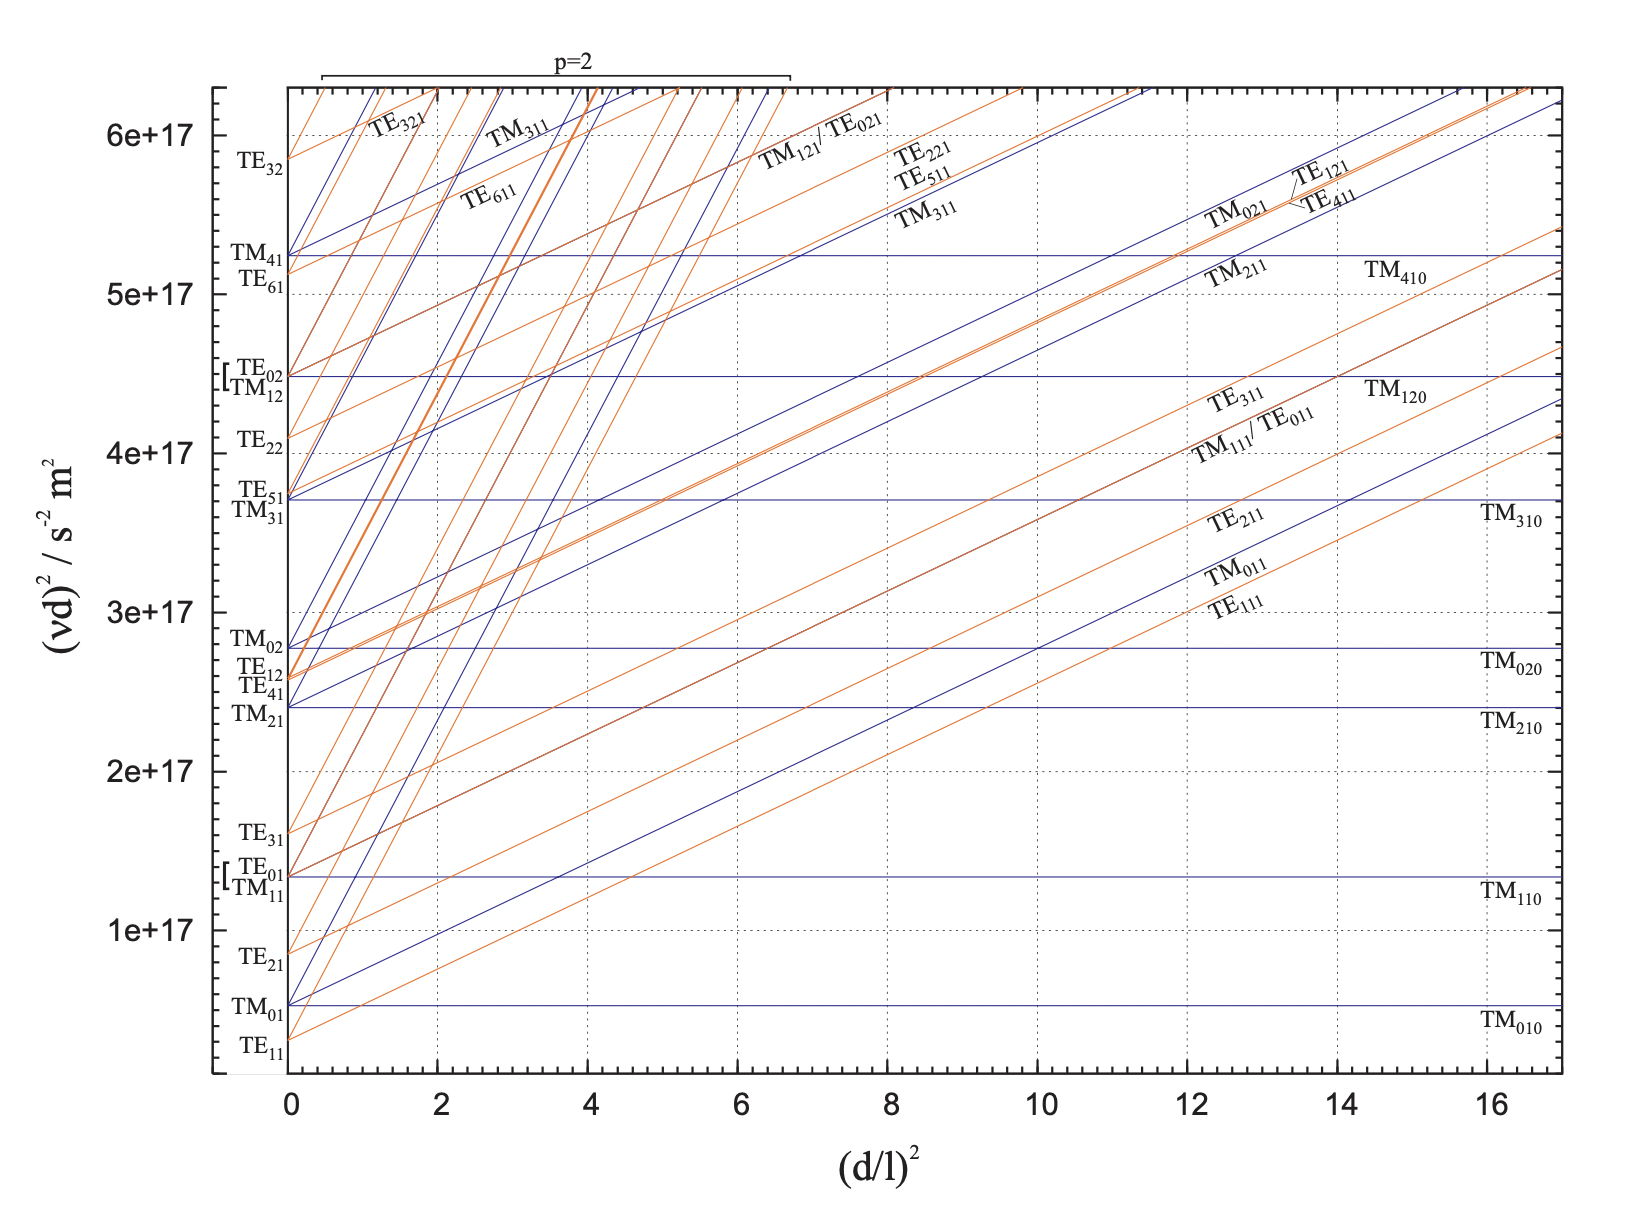
\includegraphics[width=0.8\textwidth]{mode_map}
	\caption{Mode map for $p \leq 2$. \cite{Hillert}}
    \label{fig:mode}
\end{figure}

Since the derivative of the zeroth order Bessel function and the first order
Bessel function, $j^{'}_{0n}$ and $j_{1n}$, are equal, the corresponding TE- and
TM-modes have the same resonant frequencies. That is, TE$_{0np}$-modes and
TM$_{1np}$-modes have the same resonant frequency. 

In linear accelerators and accelerating resonators to accelerate ultra-relativistic particles, the TM$_{01}$ mode is used. 
\section{Oscillating circuit}
A cavity has a lot of characteristic quantities, which can be described by an
equivalent circuit (Fig.\ref{fig:circuit}). 
\begin{figure}[hbt!]
    \centering
    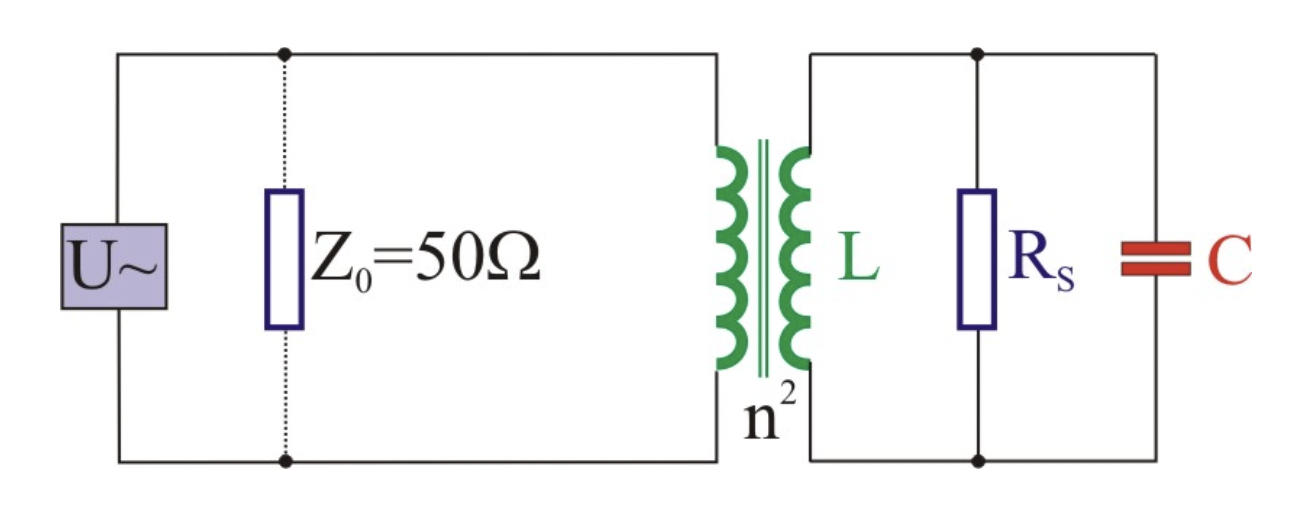
\includegraphics[width=0.8\textwidth]{circuit}
	\caption{Equivalent circuit of a cavity with loop coupling. \cite{Hillert}}
    \label{fig:circuit}
\end{figure}	

Coupling is a process through which electromagnetic waves can be coupled to a
waveguide, or in this case, to a cavity. There are several ways to couple and in
this experiment, we use loop coupling, which enables coupling to the magnetic
field inside the cavity. In the figure \ref{fig:circuit}, the LCR-circuit
represents the cavity. The step-down transformer represents the loop coupling,
$Z_{0}$ is the characteristic impedance and $R_{s}$ is the Shunt impedance. 

The characteristic quantities associated with the cavity are:
\begin{itemize}
		\item Quality factor 
		\item Coupling coefficient 
		\item Reflection coefficient 
		\item Shunt impedance
\end{itemize}

Let us look at these quantities in a bit more detail. 

\subsection{Quality factor}
Quality factor is a dimensionless quantity which describes how underdamped an
oscillator or resonator is. It is defined as: 
\begin{equation}
		Q_{0} = \frac{2 \cdot \pi \text{stored energy} }{\text{losses per period}} = \frac{2 \pi \cdot W }{T\cdot P} =  \frac{\omega_{0}\cdot W}{P}
\end{equation}
where $\omega_{0}$ is the angular resonant frequency. Looking at the case of
driven oscillations, the unloaded quality factor can be determined from the Full
Width Half Maximum (FWHM), $\Delta \omega_{H}$

\begin{equation} \label{eqn:fwhm}
		Q_{0} = \frac{\omega_{0}}{\Delta \omega_{H}}
\end{equation}

\subsection{Coupling coefficient}
The coupling coefficient is defined as:
\begin{equation} \label{eqn:coupling}
		\kappa = \frac{Z_{a}}{Z_{0}} = \frac{R_{s}}{n^2Z_{0}} = \frac{Q_{0}}{Q_{ext}}	
\end{equation}
where $n$ is the transformer turn ratio, $Q_{0}$ is the unloaded quality factor
and $Q_{ext}$ is the external quality factor.  
If we know the coupling coefficient, the unloaded quality factor can be
calculated using: 

\[
		\frac{1}{Q} = \frac{1}{Q_{0}} + \frac{1}{Q_{ext}}
\]

\begin{equation} \label{eqn:quality}
		Q_{0} = \left(1 + \kappa\right)\cdot Q
\end{equation}
\\
We also get 3 cases for the coupling coefficient, which are: 
\begin{itemize}
		\item $\kappa < 1$: undercritical coupling, $Q>Q_{0}/2$
		\item $\kappa = 1$: critical coupling, $Q = Q_{0}/2$ (no reflection)
		\item $\kappa > 1$: overcritical coupling, $Q<Q_{0}/2$ 
\end{itemize}

\subsection{Reflection coefficient}
In the conductor, we have an incoming wave ($\hat{U}_{+}, \hat{I}_{+}$) and
reflected wave ($\hat{U}_{-}, \hat{I}_{-}$). Hence we define the complex
reflection coefficient as:

\begin{equation} \label{eqn:refleccoeff}
		\rho = \frac{\hat{U}_{-}}{\hat{U}_{+}}
\end{equation}

The coupling coefficient and the reflection coefficient are related at resonance
by: 
\\
\begin{equation}
		\kappa = \left|\frac{1 + \rho}{1 - \rho} \right| 
\end{equation}
\\
We shall discuss more about this in the next section.

\subsection{Shunt impedance}
Shunt impedance tells us how much energy is gained by a charged particle when it
crosses the cavity. It is defined by: 

\begin{equation} \label{eqn:shunt}
		R_{s} = \frac{U^2}{2 P_{V}} = \frac{1}{P_{V}} \left|\int\limits_{L/2}^{-L/2} E_{0}\left(s \right) \cdot e^{i \omega_{0}s/c}\cdot ds \right|^2 
\end{equation}
\\
The impedance of the resonator in fig.\ref{fig:circuit} is a complex quantity. This value only becomes real at resonance and when it does, it is called the Shunt impedance. This value is typically of the order of $10^{6} \  \Omega$. This is the reason we use a step down transformer in the circuit, using loop coupling, as seen in Eq.(\ref{eqn:coupling}). 

\section{Scalar measurement of reflection coefficient}
The reflection coefficient we defined in the previous section (eqn. \ref{eqn:refleccoeff}) is a complex value. It looks like:

\[
		\rho(\Delta \omega) = \rho_{0} (\Delta \omega) \cdot e^{-2ikl} = \frac{\kappa - \left(1 + 2iQ_{0}\frac{\Delta \omega}{\omega}\right)}{\kappa + \left(1 + 2iQ_{0}\frac{\Delta \omega}{\omega}\right)} \cdot e^{-2ikl}
\]
\\
We get this when we investigate only take $\Delta \omega \ll \omega_{0}$. When this reflection coefficient is measured some distance $l$ away from the cavity, we get the delay factor of $e^{-2ikl}$.
\\ \\
Now, we can separate the real and imaginary part and get its modulus: 

\begin{equation} \label{eqn:scalar}
			\left| \rho (\Delta \omega) \right| = \left| \rho_{0}(\Delta \omega) \right| = \sqrt{\frac{(\kappa - 1)^2 + 4Q_{0}^2 \left(\Delta \omega / \omega \right)^2}{(\kappa + 1)^2 + 4Q_{0}^2 \left(\Delta \omega / \omega \right)^2}} 
\end{equation}
\\
The scalar network analyzer should then look like fig. \ref{fig:scalar}.

\begin{figure}[hbt!]
    \centering
    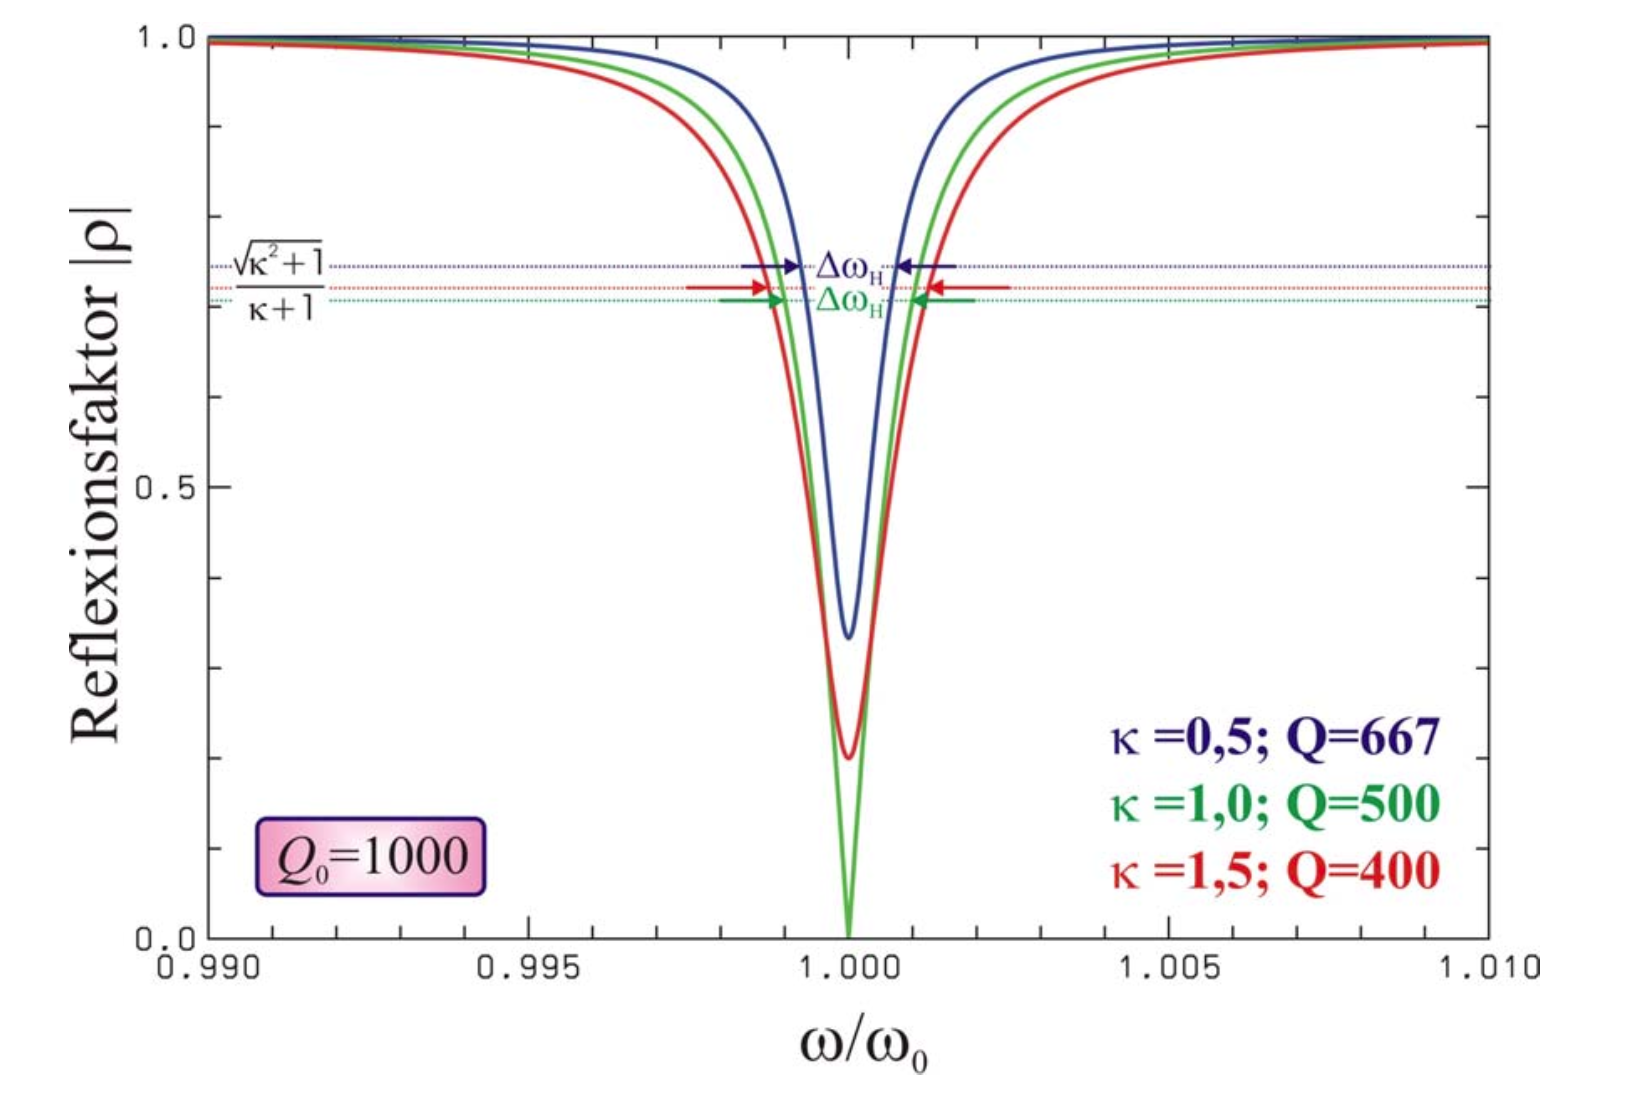
\includegraphics[width=0.8\textwidth]{scalar}
	\caption{Reflection coefficient for different values of coupling coefficient and Quality factors along with FWHM ($\Delta \omega_{H}$). \cite{Hillert}}
    \label{fig:scalar}
\end{figure}

From the figure, we can see that the reflection is minimum at resonance. At resonance, the value of the reflection coefficient is given by:

\begin{equation}
		\left| \rho (\Delta \omega = 0) \right| = \left| \frac{\kappa - 1}{\kappa +1} \right| 
\end{equation}

The equation can be inverted to calculate the value of coupling coefficient as
such:

\begin{equation}
	\kappa = 
	\begin{cases}
		\frac{1 + |\rho|}{1 - |\rho|} :& \rho > 0\\
		\frac{1 - |\rho|}{1 + |\rho|} :& \rho < 0
	\end{cases}
	\label{eqn:kappa_rho}
\end{equation}

As such, one cannot distinguish between $\rho >0$ and $\rho<0$. 

In order to calculate the value of reflection coefficient at FWHM, we use the following relation (which one can derive by using eqn.(\ref{eqn:fwhm}), (\ref{eqn:quality}) and (\ref{eqn:scalar}):

\begin{equation}
		\left| \rho (\Delta \omega_{H}/2) \right| = \frac{\sqrt{\kappa^2 + 1} }{\kappa +1} 
		\label{eqn:rho_fwhm}
\end{equation}

It is important to note that only the case of $\kappa = 1$ do we get the FWHM at $\rho = 1 / \sqrt{2} $. This is because of the way we define dB-values, which will be discussed in another section. \\
In all other cases, 

\[
		\left| \rho (\Delta \omega_{H}/2) \right| = \frac{\sqrt{\kappa^2 + 1} }{\kappa +1} \ne \frac{1}{\sqrt{2} } 
\]

The (loaded) quality factor $Q$ is then determined by following Eq.
\ref{eqn:fwhm}:
\begin{equation}
	Q = \frac{\omega_0}{\Delta\omega_H}
	\label{eqn:Q_scalar}
\end{equation}

The unloaded quality factor can easily be determined from Eq. \ref{eqn:Q_scalar}
above:
\begin{equation}
	Q_0 = (1 + \kappa)Q
	\label{eqn:Q0_scalar}
\end{equation}

\section{Vectorial measurement of reflection coefficient}
The vectorial reflection coefficient is given by: 

\begin{equation}
		\rho (\Delta \omega) = \frac{(\kappa - 1)^2 - 4Q_{0}^2 \left(\Delta \omega / \omega \right)^2 - 4i \kappa Q_{0} \Delta\omega / \omega}{(\kappa + 1)^2 + 4Q_{0}^2 \left(\Delta \omega / \omega \right)^2}  \cdot e^{-2ikl}
\end{equation}
\\
Neglecting the delay coefficient term, $e^{-2ikl}$, we get an equation, which when plotted on the complex plane (close to the resonance), $\rho_{0}$ describes a circle of radius r around ($x_{0}, y_{0}$).  The radius r is given by: 

\[
		r = \frac{\kappa}{1+ \kappa}
\]

We find that all the positions of circles are independent of quality factor and depend only on the coupling coefficient. Another interesting thing we find is that all these circles go through (-1, 0) (as shown in fig. \ref{fig:circles}). 

\begin{figure}[hbt!]
    \centering
    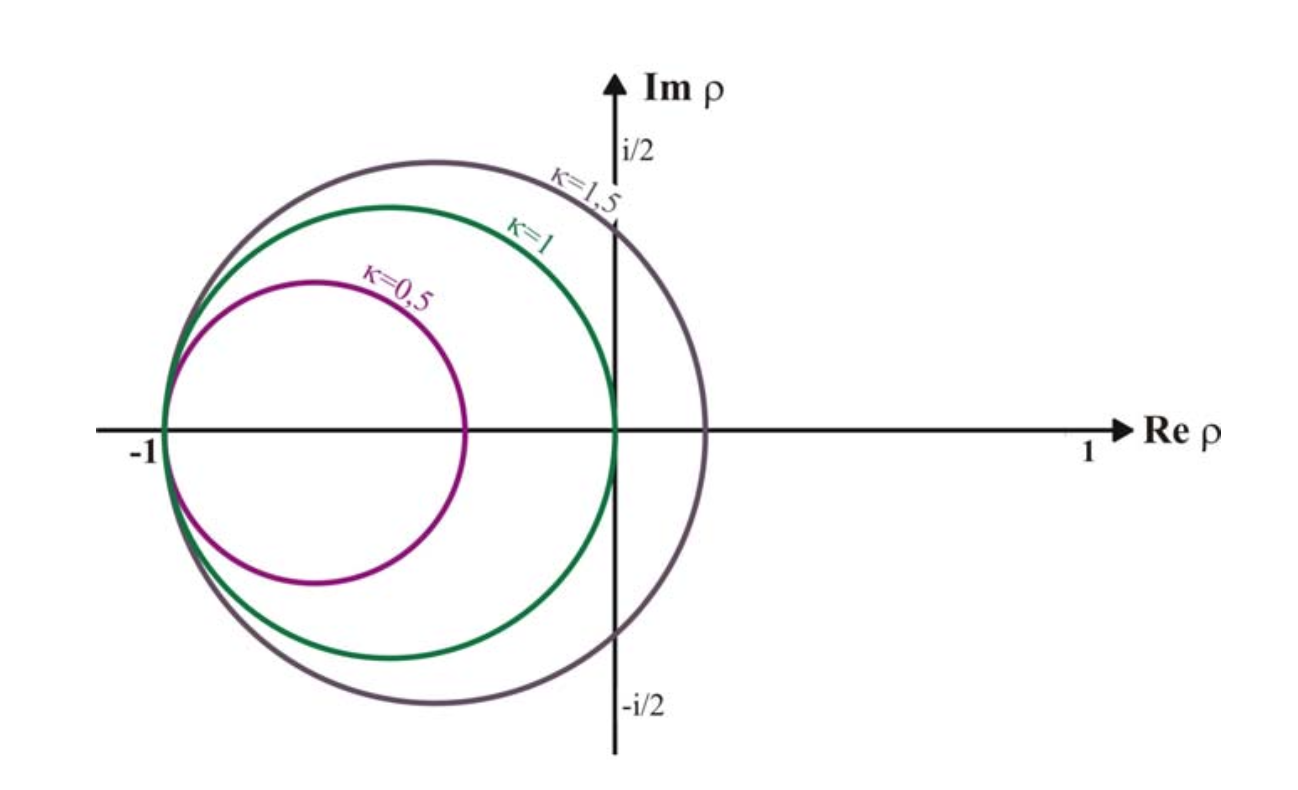
\includegraphics[width=0.8\textwidth]{circles}
	\caption{Different position and radii for different values of $\kappa$. \cite{Hillert}}
    \label{fig:circles}
\end{figure}

Now taking the delay coefficient into account, we see the circles rotate around the origin (fig. \ref{fig:delay}). For large values of quality factor, the distortion in the shape of the circle is negligible, but it is quite noticeable in low values of quality factor. We will be neglecting these distortions in our measurements because we such calibrations can be done only on expensive equipments. \\
In fig. \ref{fig:delay}, we also notice that we have an outer circle which is the reflection circle. It represents complete reflection of frequencies far away from the resonance one. The smaller circle is called the resonance circle. 

\begin{figure}[hbt!]
    \centering
    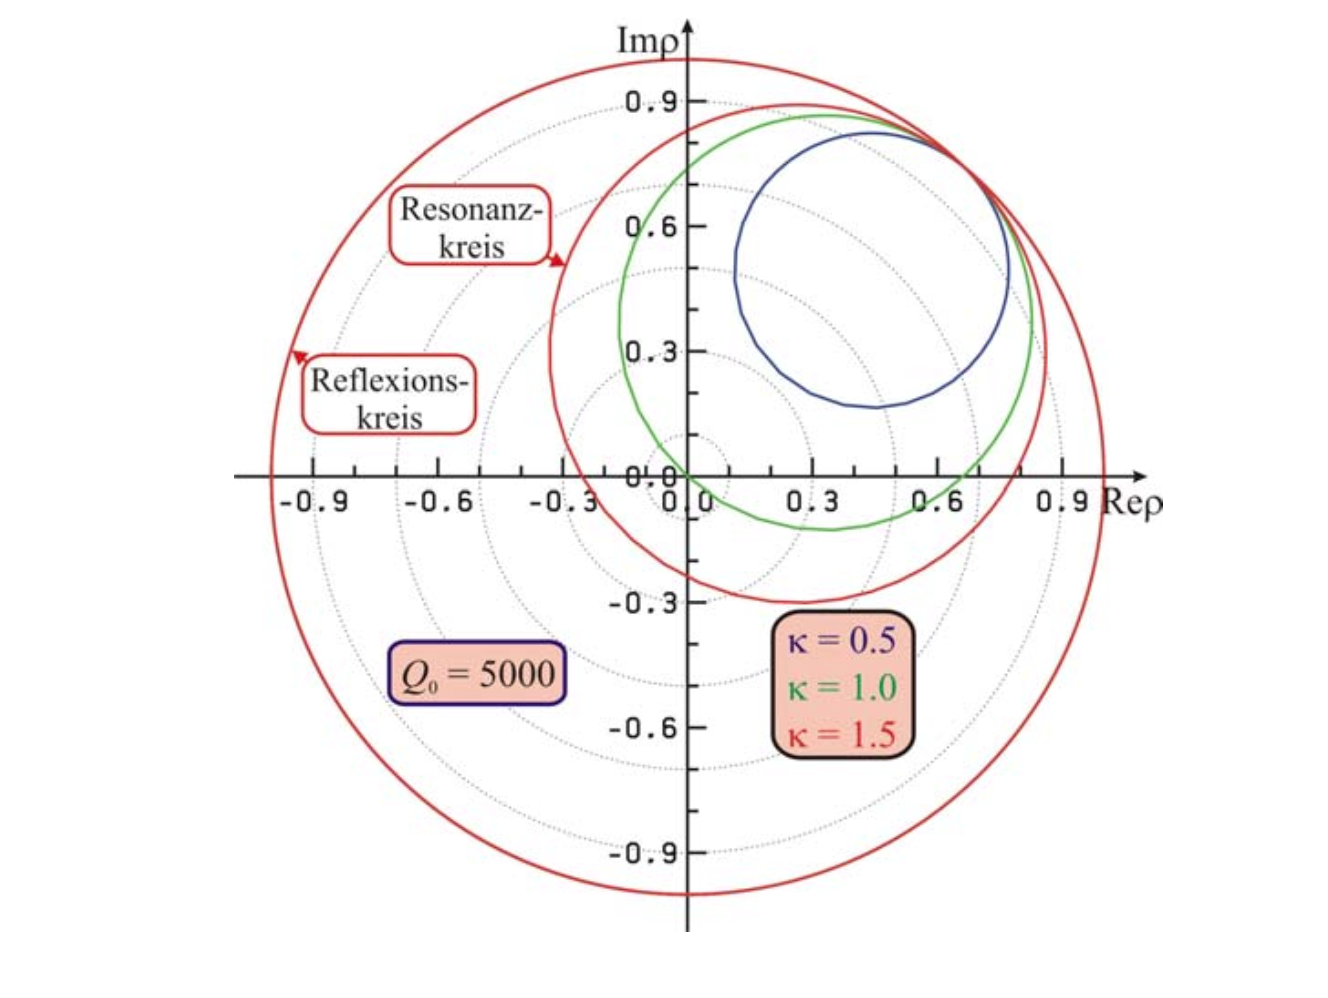
\includegraphics[width=0.8\textwidth]{delay}
	\caption{The delay coefficient rotates the circle around the origin. We can also see the Resonance and Reflection circle. \cite{Hillert}}
    \label{fig:delay}
\end{figure}

\subsection{Determining resonant frequency and coupling}
In the Vectorial Network Analyzer (VNA), we see something similar to Fig. \ref{fig:delay}. In order to determine the reflection coefficient, we rotate the circles around the origin such that the point of intersection of the resonant circle and reflection circle is on (-1, 0). Since the impedance of the resonator is real at resonance, the curve has to cross the real axis. Therefore, the point at which the resonance circle meets the real axis is the resonance frequency $\omega_{0}$. \\
In order to determine the reflection coefficient, we simply look at the distance between the resonant point and the origin, $d$, and the radius of the reflection circle, $R$. The reflection coefficient is then defined as: 

\[
		\rho_{0} = d/ R
\]

The coupling coefficient is given by: 

\[
		\kappa = \frac{1 + \rho_{0}}{1 - \rho_{0}}
\]


\subsection{Determining quality factor}
Similar to the scalar measurement, we use

\[
		\frac{\Delta \omega_{H}/2}{\omega_{0}} \approx \frac{1 + \kappa}{2Q_{0}}	
\]

and we get 

\[
		\rho_{0}(\pm \Delta \omega_{H}/2) = -\frac{1}{\kappa + 1} \mp i\frac{\kappa}{\kappa + 1}
\]

Therefore, the frequency shift $\Delta \omega$ from the resonant frequency and hence the FWHM can be determined by the intersection of the resonance circle around (0, $\pm i/2$).
This is essentially the frequency that is $\pi / 2$ rotation away from the resonant frequency on the resonance circle. 

\subsection{Determining Power Loss}

The power loss in the cavity $P$ can be determined by utilizing the Smith diagram with the reflections circles to 
determine the standing wave ratio. The standing wave ratio (SWR) quantifies the degree of reflection of a signal. It is ranged
from $[1, \infty)$ such that for SWR $\rightarrow 1$ the signal is totally reflected, and for
SWR $\rightarrow \infty$, the signal is totally transmitted (i.e. no reflections are observed). The SWR can be
described as such: 
\begin{equation}
	S = \frac{|\hat{U}_{max}|}{|\hat{U}_{min}|} = \frac{1 + |\rho|}{1 - |\rho|}
\end{equation}

The power dissipation in the resonator can then be described as such: 

\begin{equation} \label{eqn:power_loss}
	P = \frac{4S}{(1 + S)^2} P_0
\end{equation}

where $P_0$ is the input power of the signal. 

\section{Bead pull measurement}
In order to measure the electric and magnetic field inside the cavity, we cannot use an antenna because that would disturb the field distribution inside. Instead, we introduce a small bead inside the cavity, a small perturbation. This bead, which is usually a dielectric or a conducting object, causes a shift in the resonant frequency, which can be measured. It can also be fixed with a constant excitation with $\omega_{0}$ and the change in reflection coefficient can be observed. These two things can be used to determine the fields inside the cavity. 

\subsection{Resonant bead pull measurement}
The case in which we measure the shift in the resonant frequency is called resonant bead pull measurement. A small teflon bead ($\epsilon_{r}$ = 2.1 , $r$ = 1mm) is moved in small increments inside the cavity. For each increment, the we get a shift in the resonance frequency $\Delta \omega(z)$. The Electric field, $E_{0}(z)$ is given by:

\begin{equation} \label{eqn:E0_res}
		E_{0}(z) = \sqrt{2 \cdot \frac{W}{\alpha_{S}}\cdot \frac{\Delta \omega(z)}{\omega_{0}}}
\end{equation}
where $\alpha_{s}$ is the perturbing constant: 

\[
		\alpha_{S} = \frac{1}{2} \cdot (\epsilon - \epsilon_{0}) \cdot V_{S}
\]
$V_{S}$ is the volume of the bead. 

\subsection{Non-resonant bead pull measurement}
The case in which we measure the change in reflection coefficient without changing the excitation is called non-resonant bead pull measurement. The electric field is determined by: 

\begin{equation} \label{eqn:E0_nonres}
		E_{0}(z) = \sqrt{\frac{(1 + \kappa)^2}{2 \kappa Q_{0}}\cdot \frac{W}{\alpha_{S}}\cdot \left| \Delta \rho(z) \right| }
\end{equation}

\subsection{Shunt impedance}
For determining the shunt impedance, it is sufficient to know the electric field. The accelerating voltage $U$ is given by: 

\[ 
		U = \int\limits_{0}^{L} E_{0}(z) \cdot dz
\]
Using this and Eqn. \ref{eqn:shunt}, we can define a delay coefficient as: 

\begin{equation}
		\Lambda = \left| \frac{\int\limits_{-L/2}^{L/2} E_{0}(s) \cdot e^{i \frac{\omega_{0}s}{c}\cdot ds}}{\int\limits_{-L/2}^{L/2} E_{0}(s) \cdot ds} \right| = 
		\left| \frac{\int\limits_{-L/2}^{L/2} E_{0}(s) \cdot \cos\left(\frac{\omega_{0}s}{c} \right)\cdot ds }{\int\limits_{-L/2}^{L/2} E_{0}(s) \cdot ds} \right| 
\end{equation}

where the time transit factor $e^{i \frac{\omega_{0}s}{c}} = \cos\left(\frac{\omega_{0}s}{c}\right)$ as we are dealing with real values of frequencies. \par 
And finally, we have for resonant method:

\begin{equation} \label{eqn:Rs_res}
		R_{s} = \Lambda \cdot \frac{2Q_{0}}{\omega_{0}^2 \cdot \alpha_{S}} \cdot \left| \int\limits_{-L/2}^{L/2} \sqrt{\Delta \omega (z)} \cdot dz \right|^2
\end{equation}

And for non-resonant method we have: 

\begin{equation} \label{eqn:Rs_nonres}
		R_{s} = \Lambda \cdot \frac{(1 + \kappa)^2}{2 \omega_{0} \kappa \alpha_{S}} \cdot \left| \int\limits_{-L/2}^{L/2} \sqrt{\Delta \rho (z)} \cdot dz \right|^2
\end{equation}

The energy gain of a particle accelerating within a cavity can then be defined using Eq. \ref{eqn:shunt}, considering that the power dissipation due to the cavity 
can be related to the measured power $P_v = P / (1 + \kappa)$ as follows:
\begin{equation} \label{eqn:energy_gain}
	\delta U = \sqrt{\frac{2 R_s P}{1 + \kappa}}
\end{equation}\
This will be used to determine the efficiency of the cavity for particle acceleration.

\section{dB and DBm}
Decibel (symbol: dB), is logarithmic quantity that indicated gain or loss, with respect to a reference value. It is defined as: 

\begin{equation}
		L_{P} = 10  \log_{10}\left(\frac{P}{P_0}\right) \ dB
\end{equation}
where $P$ is the measured power and $P_{0}$ is the reference power. When we take this reference power $P_{0}$ = 1mW, it is known as decibel-milliwatts (dBm). It is defined as: 

\begin{equation}
		L_{P} = 10 \log_{10} \left(\frac{P}{1 mW}\right) \ dBm
\end{equation}

When talking about root-power quantities (for instance voltage and current), the ratio of the squares is taken.

\begin{equation} \label{eqn:db}
		L_{F} = 10 \log_{10} \left(\frac{F^2}{F_{0}^2}\right) \ dB = 20 \log_{10} \left(\frac{F}{F_{0}}\right) \ dB
\end{equation}

Recalling our discussion from before, about the FWHM, in Eq. \ref{eqn:rho_fwhm}, we see that only in the case where $\kappa = 1$ do we get the full 3dB-FWHM, corresponding to the value $\rho = 1/\sqrt{2}$. This is because of how dB is defined in the Eq. \ref{eqn:db}.  

\chapter{Exercise before the experiment}

In this pre-lab exercise, we estimate the frequency for various modes of the cavity by using the mode map (Fig. \ref{fig:mode}) and using the Eq. \ref{eqn:res_freq}. The cylindrical cavity has an inner diameter of 78.5mm and length of 20mm. 
So we have, $\left(d/l\right)^2 = 15.405625$. Therefore, from the mode map, the ten lowest eigenmodes are tabulated in the table \ref{tab:mode_freq1}. 

\begin{table}[htpb]
		\centering
		\caption{Eigenmodes and their corresponding frequencies calculated using the mode map.}
		\label{tab:mode_freq1}
		\begin{tabular}{|c|c|}
				\hline Eigenmodes &  Frequency (GHz) \\
				\hline $TM_{010} $ & 2.848 \\
				\hline $TM_{110} $ & 4.593 \\
				\hline $TM_{210} $ & 6.240 \\
				\hline $TM_{020} $ & 6.740 \\ 
				\hline $TE_{111} $ & 7.643 \\ 
				\hline $TM_{310} $ & 7.748 \\
				\hline $TM_{011} $ & 7.955 \\ 
				\hline $TE_{211} $ & 8.353 \\
				\hline $TM_{120} $ & 8.545  \\
				\hline $TM_{111}/TE_{011}$ & 8.733 \\
				\hline		
		\end{tabular}
\end{table}

The values calculated using Eq. \ref{eqn:res_freq} is shown in the table \ref{tab:mode_freq2}.

\begin{table}[htpb]
		\centering
		\caption{Eigenmodes and their corresponding frequencies calculated using the formula.}
		\label{tab:mode_freq2}
		\begin{tabular}{|c|c|}
				\hline Eigenmodes & Frequency (GHz) \\ 
				\hline $TM_{010} $ & 2.925 \\
				\hline $TM_{110} $ & 4.661 \\
				\hline $TM_{210} $ & 6.247 \\
				\hline $TM_{020} $ & 6.715 \\ 
				\hline $TE_{111} $ & 7.827 \\ 
				\hline $TM_{310} $ & 7.761 \\
				\hline $TM_{011} $ & 8.050 \\ 
				\hline $TE_{211} $ & 8.369 \\
				\hline $TM_{120} $ & 8.534  \\
				\hline $TM_{111}/TE_{011}$ & 8.830 \\
				\hline	
		\end{tabular}
\end{table}


\chapter{Setup and Procedure}

\section{Experimental Setup}

In our experiment, we used three cylindrical cavities, each with a length of
$L_{cav} = \SI{20}{\milli\metre}$ with an inner diameter of $d_{cav} =
\SI{78.5}{\milli\metre}$. The first and second cavity are completely sealed and
are free to move, but differ in their coupling position to the radio frequency.
The third cavity is open from the sides and is mounted on a rail, in which its
position can be freely adjusted and is displayed on an external device
digitally. A thread with a teflon bead of radius $r_{bead} = \SI{1}{\milli\metre}$ and
relative permittivity of $\epsilon_{r, bead} = 2.1$ was placed on the same
mount such that the bead can pass through the cavity. The cavities used are shown in Fig.
\ref{fig:cavities_equipment}.

\begin{figure*}[hbt!]
	\centering
	\subfloat[\centering
	\label{fig:top_cavity}]{{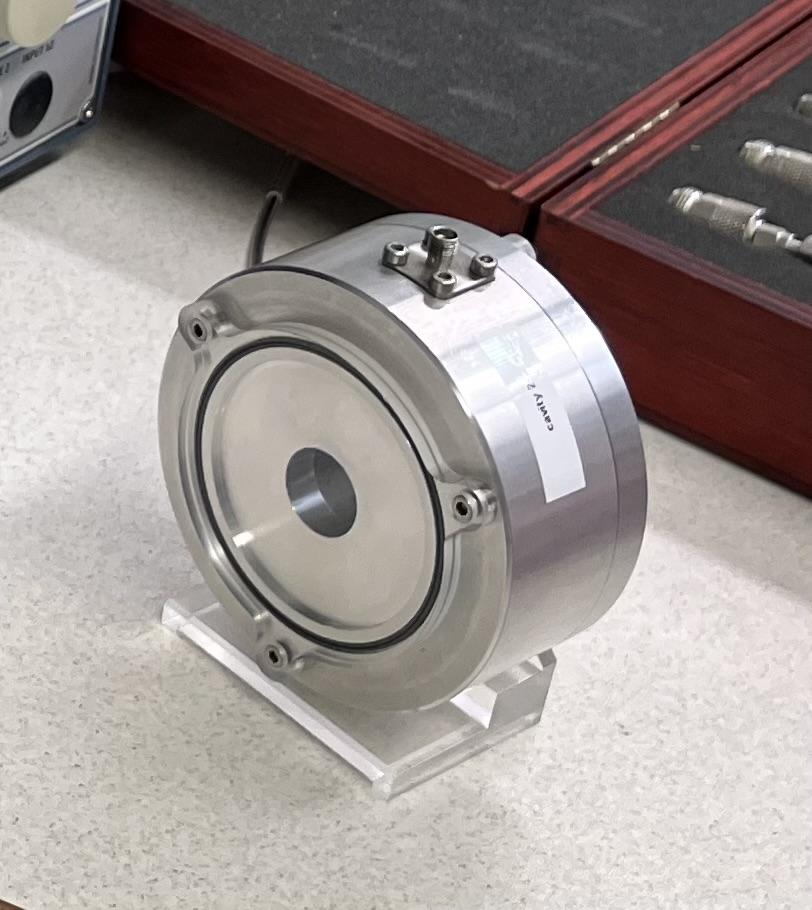
\includegraphics[width=0.3\columnwidth]{cavity_top.jpg}}}
	\quad
	\subfloat[\centering
	\label{fig:mounted_side_cavity}]{{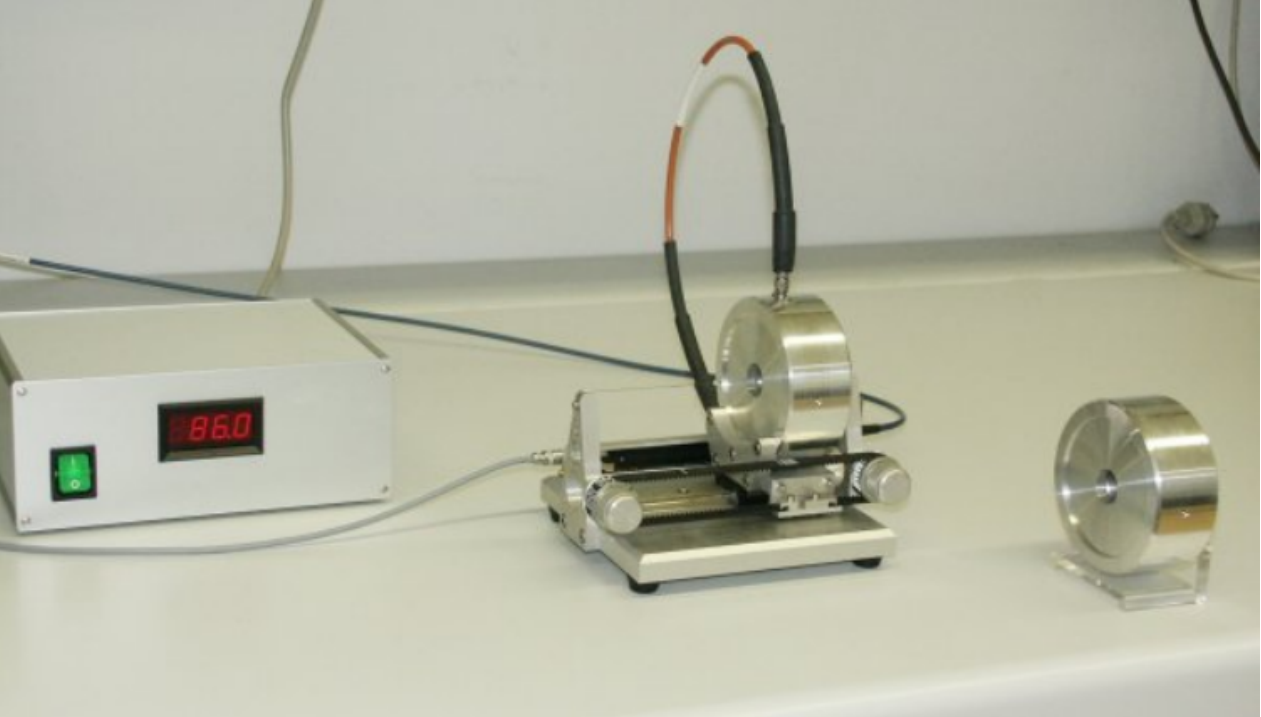
\includegraphics[width=0.6\columnwidth]{cavity_side_rail.png}}}

	\caption{The three cavities used in this experiment. (a): The cavity with
	top coupling. The connector that couples the radio frequency can be
	observed. (b) The cavity with side coupling (right) and the mounted cavity
	(left) \cite*{Switka22}. The detector used to measure the position of the
	mounted cavity is also shown.}
	\label{fig:cavities_equipment}
\end{figure*}

To measure the resonant frequencies, reflection coefficients, and other relevant
quantities in our experiment, we utilize a Vector Network Analyzer (VNA) shown
in Fig. \ref{fig:VNA}. The VNA generates a signal from its AC source and it is
transmitted through the coaxial cable connected to the ports of the VNA. The
resulting transmission or reflection of the signal is then shown on the display
as a function of the frequency of the signal (in Hz). The units displayed can be
altered between $U$, the ratio between output and input signal, and $dB = 20
\log_{10}(U)$. \par  

\begin{figure*}[hbt!]
	\centering
	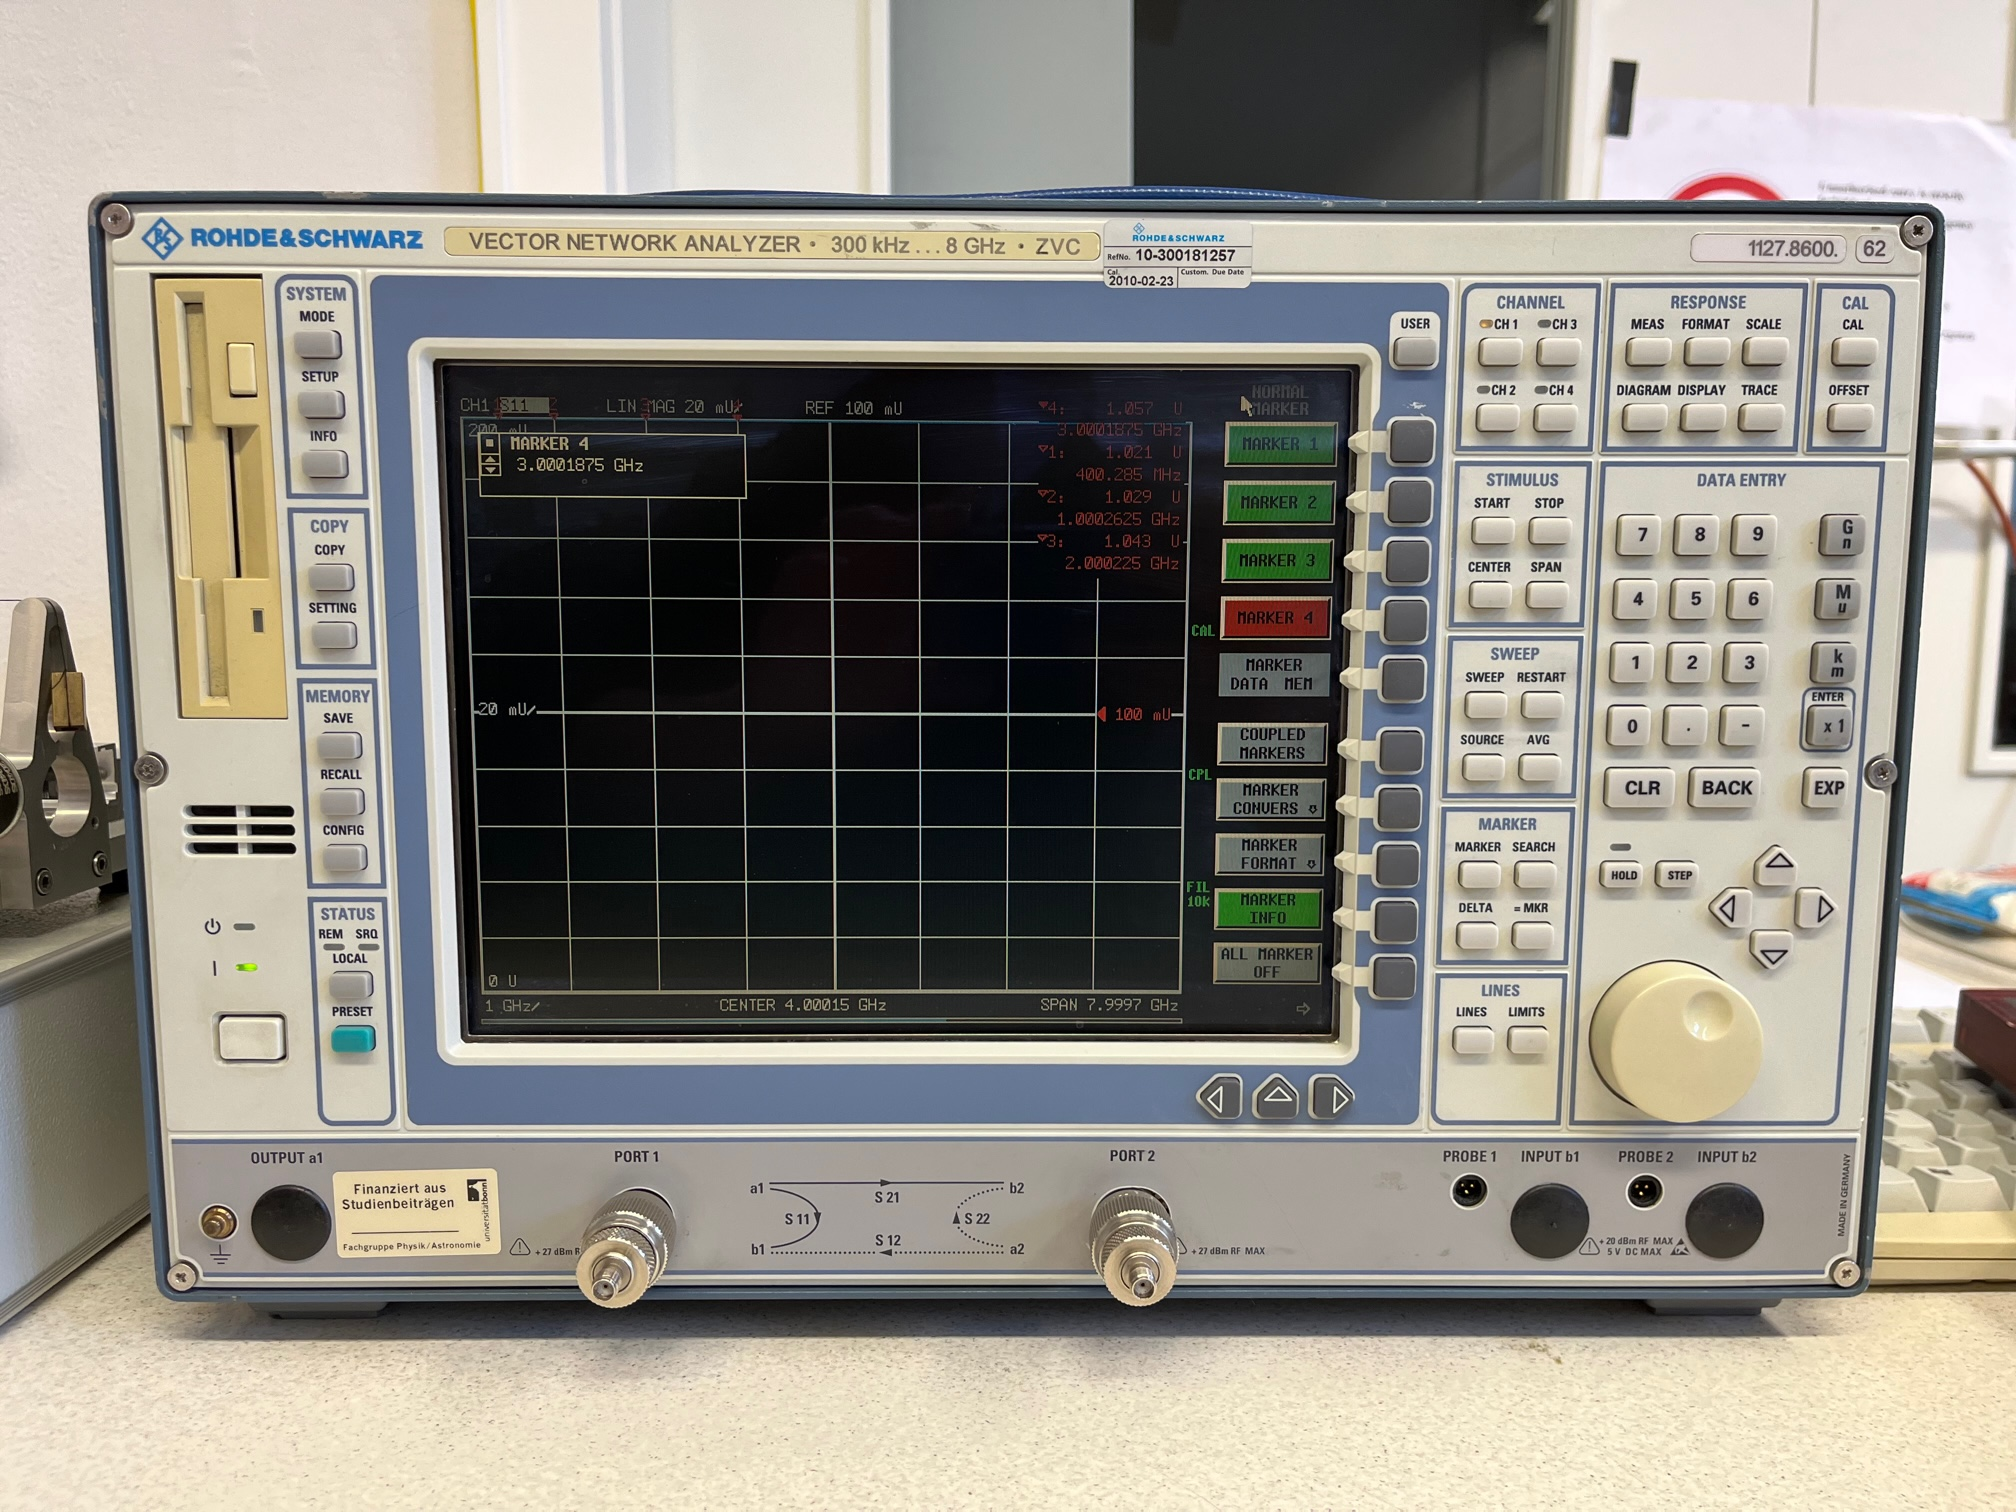
\includegraphics[width=0.5\columnwidth]{VNA.jpg}
	\caption{The Rhode \& Schwarz Vector Network Analyzer used in this experiment.}

	\label{fig:VNA}
\end{figure*}

\section{Procedure}

\subsection{Attenuation and Reflection in Coaxial Cables}

As the coaxial cable connects the cavity to the VNA, we need to choose a cable
such that it does not interfere with the measurement of the cavity's response.
To determine the optimal coaxial cable to use, we thus measured the attenuation
and reflection of different coaxial cables at different frequency ranges. In our
experiment, this was done for the RG-142 and ST-18 cables with a length of
$l_{RG142}=\SI{51.02 \pm 0.10}{\centi\meter}$ and $l_{ST18}=\SI{182.55 \pm
0.10}{\centi\meter}$ respectively. The uncertainty of the length was obtained
from the width of the scale of the measuring apparatus. \par 

To measure the attenuation and reflection, we first calibrated the VNA to the
silver RG402 coaxial cable with a length of $l_{RG402} = \SI{30.02 \pm
0.01}{\centi\meter}$. The calibration process was performed using a full-two
port calibration with the TOSM algorithm provided by the VNA. The open, short,
and load (with termination impedance of $\SI{50}{\ohm}$) at the two ports (port
2 on the VNA and the coaxial cable) were then calibrated by utilizing the
provided calibration kit (Fig. \ref{fig:calibration_kit}). 

\begin{figure*}[hbt!]
	\centering
	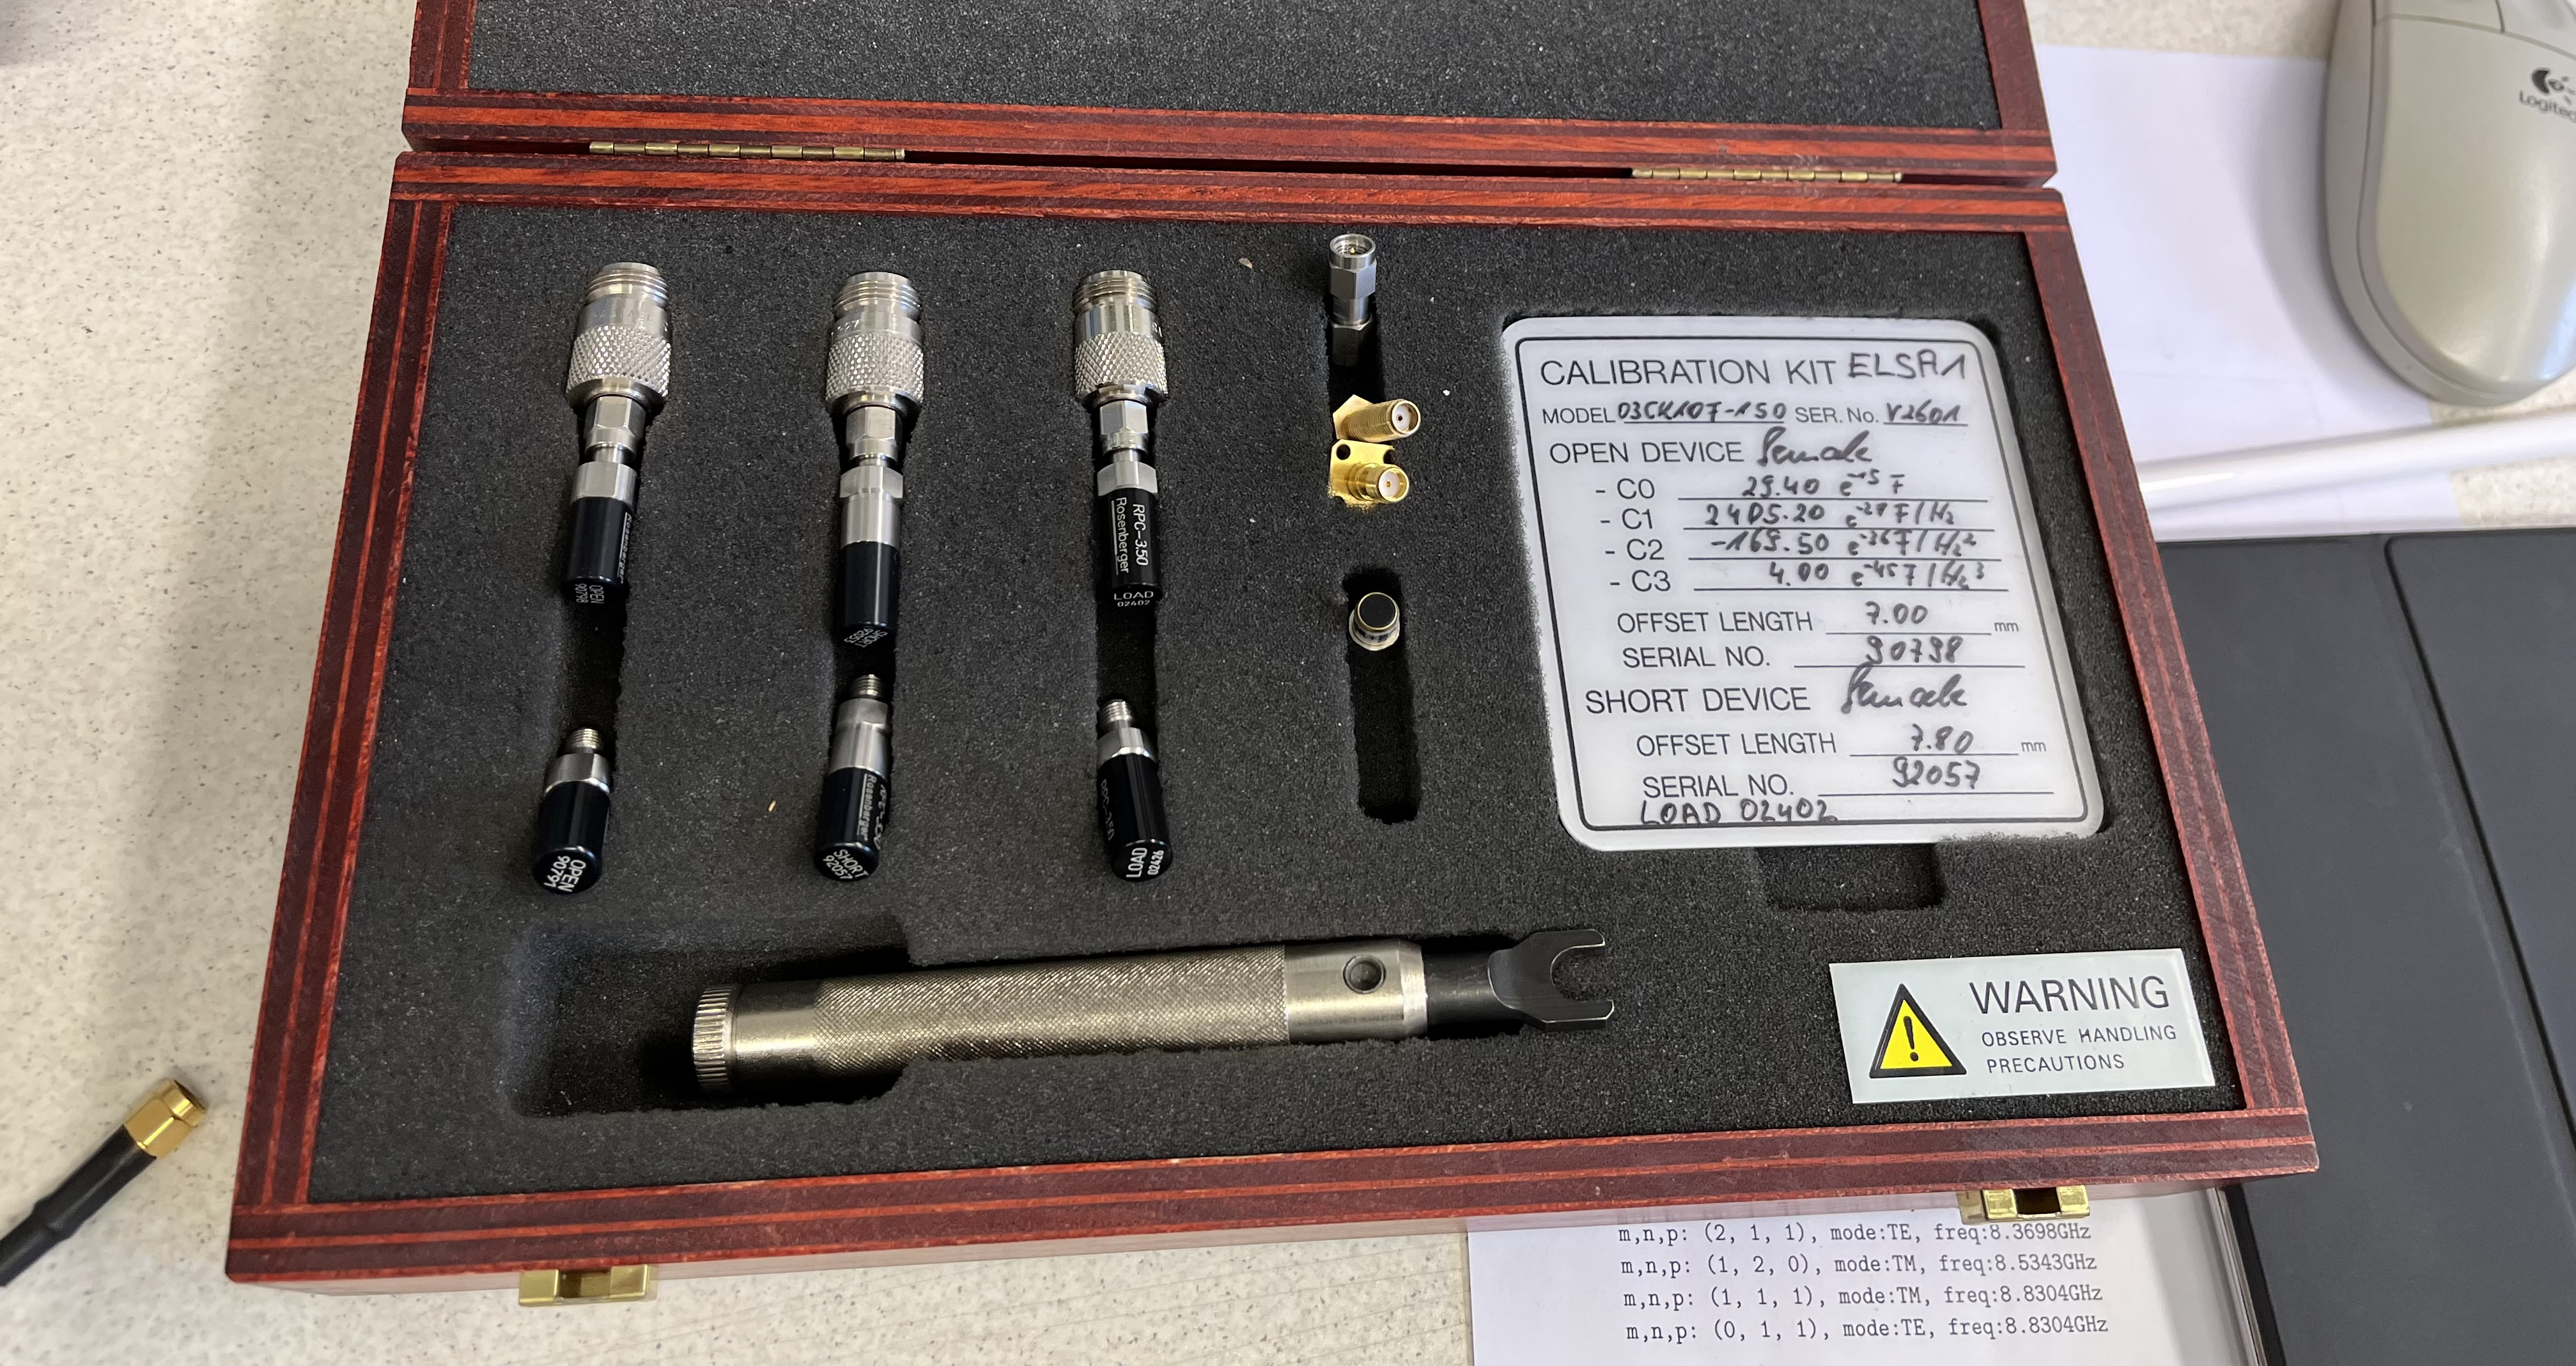
\includegraphics[width=0.6\columnwidth]{calibration_kit.jpg}
	\caption{The open (left), short (middle) and load (right) used for
			calibration in this experiment.}

	\label{fig:calibration_kit}
\end{figure*}

The attenuation of the signal was then measured by connecting the end of the
coaxial cable to the input port (port 2) on the VNA. We then connect the same
load from the calibration kit to the end of the coaxial cable to measure the
reflection coefficient. Both measurements were performed to verify that the VNA
was properly calibrated. \par 

After the calibration was performed with the silver cable, we connected the two
coaxial cables to the silver cable and measured their attenuation and reflection
coefficient by performing the same procedure as with the silver one. The raw
measurements obtained are shown in Fig.  \ref{fig:calib_raw}. The fluctuations in the signal were taken into account as the
uncertainty in the coefficients. We neglected effects due to the connector
between the two cables.

\begin{figure*}[htb!]
	\centering
	\subfloat[Transmission for the RG142 cable.
	]{{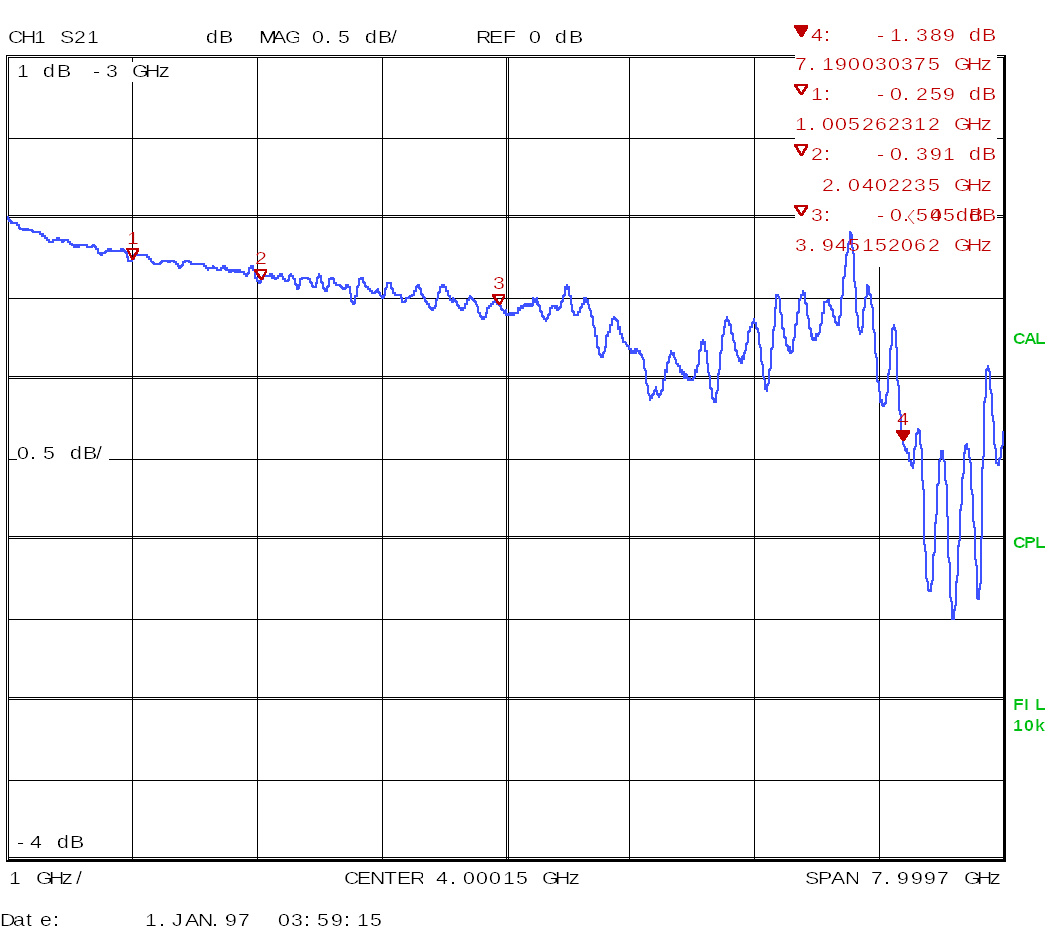
\includegraphics[width=0.48\columnwidth]{calib_brown_s21.png}}}
	\quad
	\subfloat[Transmission for the ST18
	cable.]{{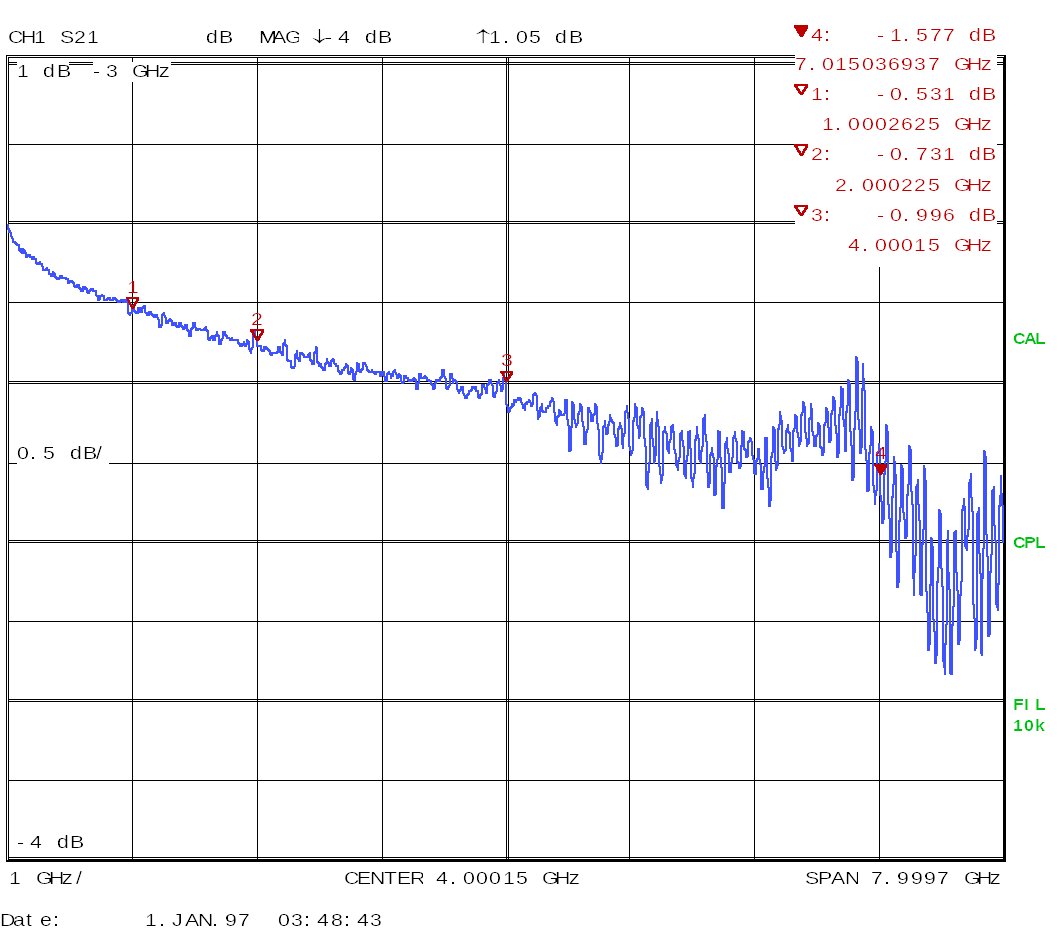
\includegraphics[width=0.48\columnwidth]{calib_blue_s21.png}}}
	\quad
	\subfloat[Reflection for the RG142
	cable.]{{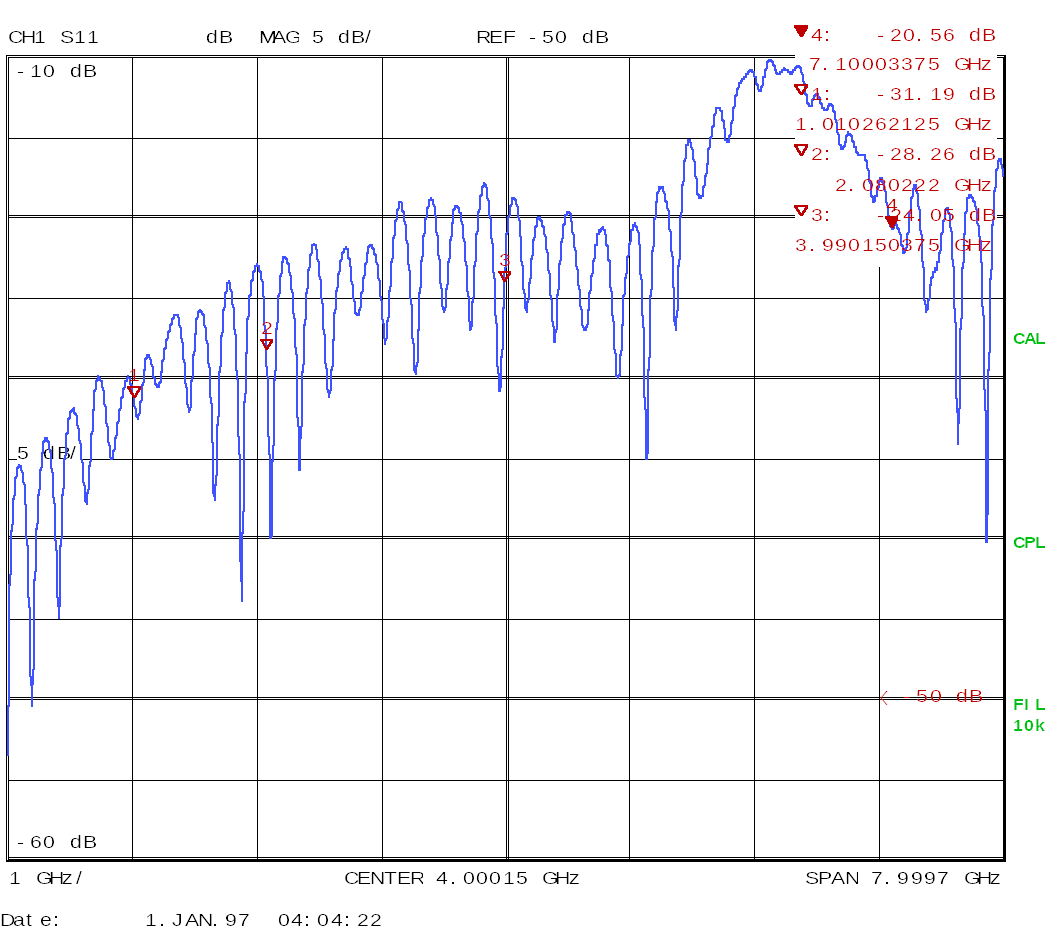
\includegraphics[width=0.48\columnwidth]{calib_brown_s11.png}}}
	\quad
	\subfloat[Reflection for the ST18
	cable.]{{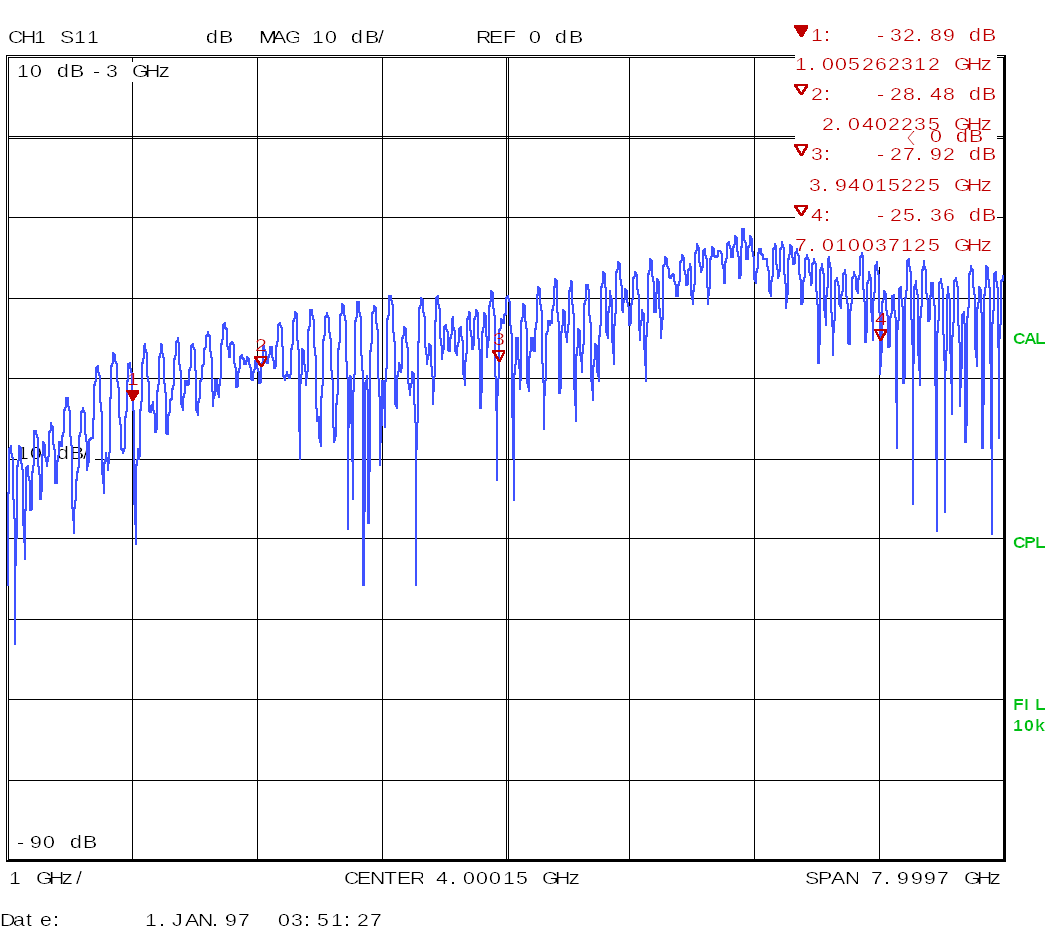
\includegraphics[width=0.48\columnwidth]{calib_blue_s11.png}}}

	\caption{The transmission and reflection for the RG142 and ST18 coaxial
	cables. The values at several frequencies are also shown on the top right of
	each figure. }
	\label{fig:calib_raw}
\end{figure*}

The transmission and reflection at several frequencies were then tabulated and were used to determine the attenuation
of the cable. The attenuation $\lambda$ (in units of dB m$^{-1}$) of a coaxial cable can be determined by the ratio of the
reflected and transmitted power $P_R$, $P_T$ as such:
\begin{equation}
	\lambda = 20 \log_{10}\left(\frac{P_{in}}{P_{out}}\right) = 20 \log_{10}\left(\frac{P_R}{P_T}\right)
\end{equation} 

The resulting attenuation was then compared to those provided in the datasheets
from the manufacturers.\par 

\subsection{Scalar Measurement}

We then connected the brown coaxial cable to the top cavity (cavity with top
coupling), and the resulting reflection coefficient was displayed on the VNA.
We then pinpointed several points in frequency in which a sharp dip in the
reflection curve was observed. Such points corresponded to 
resonant modes in the cavity. Before taking the measurement of each resonant frequency, the VNA was calibrated
using a full one-port procedure, calibration with the kit from Fig.
\ref{fig:calibration_kit} as before. An example of a resonance in the
reflection curve is shown in Fig. \ref{fig:resonance_raw}. The corresponding
reflection coefficient and resonant frequency was then measured. The
fluctuations and width of the scales taken into account as uncertainties in the
reflection coefficient. The step size of the VNA was $\SI{50}{\kilo\hertz}$, which was also considered as the
uncertainty in frequency measurements.
\par 

\begin{figure*}[htb!]
	\centering
	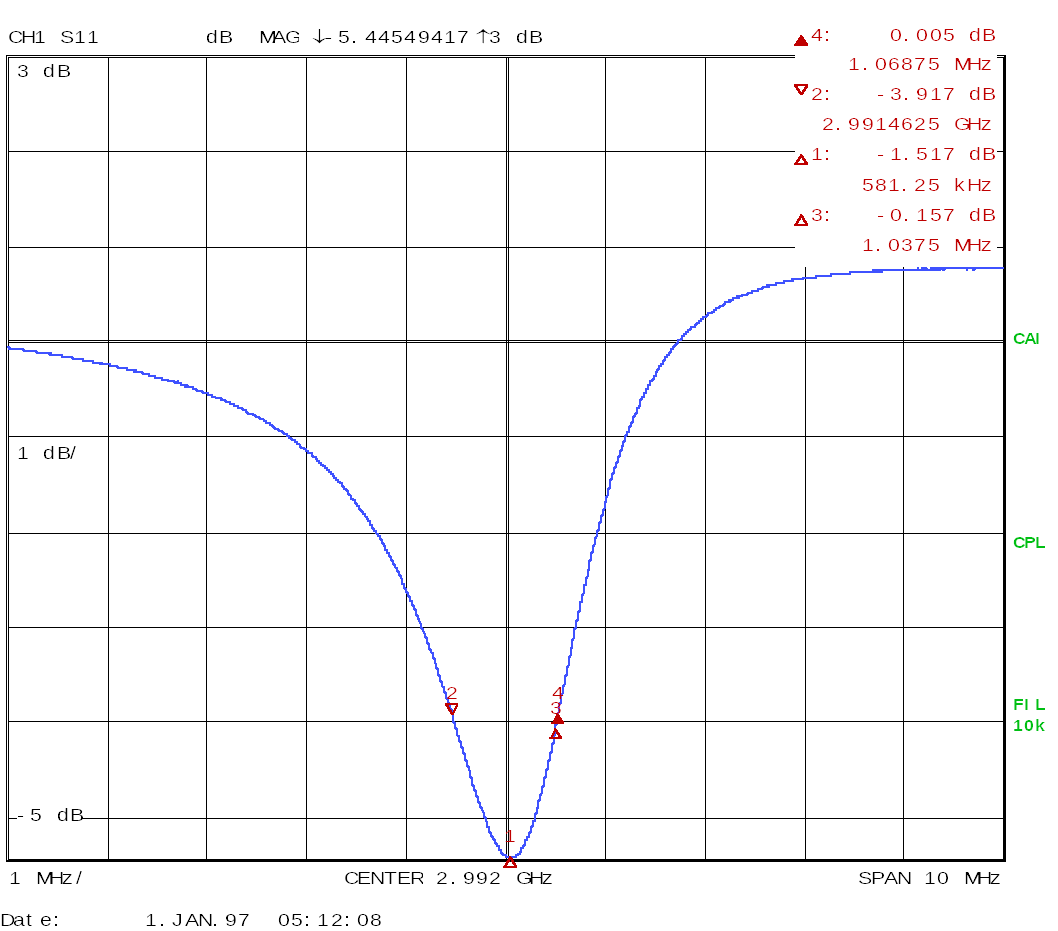
\includegraphics[width=0.6\columnwidth]{resonant1.1.png}
	\caption{Reflection curve at a resonant frequency of $\omega_0 =
	\SI{2.992206875}{\giga\hertz}$. }

	\label{fig:resonance_raw}
\end{figure*}

To obtain the full-width half-maximum (FWHM) of the curve, the reflection
coefficient obtained at resonance $|\rho(\omega_0)|$ was used to determine the
coupling coefficient as shown in Eq. \ref{eqn:kappa_rho}. The reflection
coefficient at $\frac{\Delta\omega_H}{2}$ was then evaluated by using Eq.
\ref{eqn:rho_fwhm} and the corresponding frequency values, that is, the half of the FWHM, were measured using
the display. The loaded and unloaded quality factor was then determined using Eq. \ref{eqn:Q_scalar} and
\ref{eqn:Q0_scalar} respectively. Gaussian error propagation techniques were
utilized to obtain the correct uncertainties for relevant quantities. \par 


This procedure was performed for each observed resonance peak until $\SI{8}{\giga\hertz}$, the
maximal frequency in which the VNA can measure. The same analysis was repeated
for the side cavity, and the resonant frequency obtained in both cases were
compared with the analytical resonant frequencies evaluated from Eq. \ref{eqn:res_freq}. The raw data
for both cases are presented in Table \ref{tab:raw_scalar_top} and \ref{tab:raw_scalar_side}. 

\begin{table}[htb!]
	\centering
	\begin{tabular}{|c|c|c|c|c|c|}
		\hline $\omega_0$ / GHz & $\left| \rho(\omega_0) \right|$ / dB & $\kappa$ & $\left| \rho(\Delta\omega_H / 2) \right|$ / dB & $\Delta\omega_H$ / MHz\\ 
		\hline 2.992206875 & $-5.445 \pm 0.010$ & $-1.4499 \pm 0.0010$ & $-3.915 \pm 0.015$ & 2.1375 \\ 
		\hline 4.53973125 & $-40.0 \pm 5.0$ & $-1.0513 \pm 0.0066$ & $-28.3 \pm 1.0$ & 0.575 \\
		\hline 6.21559375 & $-2.37 \pm 0.05$ & $ -2.460 \pm 0.053$ & $-1.819 \pm 0.051$ & 5.5625 \\
		\hline 6.940125 & $-9.575 \pm 0.50$ & $-1.233 \pm 0.014$ & $-6.81 \pm 0.13$ & 5.625 \\ 
		\hline 7.75975 & $-4.13 \pm 0.080$ & $-1.639 \pm 0.016$ & $-3.005 \pm 0.061$ & 8.75 \\ 
		\hline
	\end{tabular}
	
	\caption{Raw data for relevant quantities measured at resonant modes of top cavity. $\kappa$ and $\left| \rho(\Delta\omega_H / 2) \right|$ 
			are calculated quantities used to measure $\Delta\omega_H$. }
	\label{tab:raw_scalar_top}
\end{table}

\begin{table}[htb!]
	\centering
	\begin{tabular}{|c|c|c|c|c|c|}
		\hline $\omega_0$ / GHz & $\left| \rho(\omega_0) \right|$ / dB & $\kappa$ & $\left| \rho(\Delta\omega_H / 2) \right|$ / dB & $\Delta\omega_H$ / MHz\\ 
		\hline 2.98690625 & $-2.404 \pm 0.005$ & $-2.4245 \pm 0.0051$ & $-1.8411 \pm 0.0051$ & 4.0625 \\ 
		\hline 4.49725 & $-1.270 \pm 0.020$ & $-8.41 \pm 0.55$ & $-1.143 \pm 0.083$ & 1.375 \\
		\hline 6.2078875 & $-3.755 \pm 0.010$ & $ -1.7270 \pm 0.0026$ & $-2.745 \pm 0.040$ & 0.8125 \\
		\hline 7.74540625 & $-6.625 \pm 0.030$ & $-1.3556 \pm 0.0019$ & $-4.737 \pm 0.070$ & 0.875 \\ 
		\hline
	\end{tabular}
	\caption{Same as Fig. \ref{tab:raw_scalar_top} but for the side cavity. }
	\label{tab:raw_scalar_side}
\end{table}


\subsection{Vectorial Measurement}

We then used the top cavity to determine the resonant frequency and FWHM for the
first fundamental eigenmode vectorially. This was done using the reflection
curves as shown in Fig. \ref{fig:delay}, which is done by switching the display on the VNA to the complex representation. \par 

The resonant frequency was first determined by using the same method as with the
scalar analysis. We then switched to the complex representation and rotated the
curve such that the point on the curve at resonance intersects with the real
axis. The FWHM was then determined by first evaluating for the coupling
coefficient, using the same equations as with the scalar analysis. The
corresponding values of $|\rho(\frac{\Delta\omega_H}{2})|$ were then determined
on the resonant circle, and the resulting frequency values were tabulated.
The fluctuations of the measurement were again taken into account as uncertainties
in our measurement. We also recorded the input power to be $P_0 = 1.5 \pm 0.1$dB. \par 

In our measurement, the more accurate method that utilizes the distance between points on the reflection and resonant circle 
to determine the coupling coefficient was not performed due to the error in the calculated $|\rho(\frac{\Delta\omega_H}{2})|$
when using this method. This may have been resolved if we had used units of power ratios $U$ instead of dB to determine the 
coupling coefficient. This is also the reason why $\kappa$ in the scalar measurement yielded negative values. In the future,
units in the measurement should be set to $U$ as much as possible. \par 

The obtained values were then used to determine the loaded, unloaded and external quality
factor $Q$, $Q_0$, $Q_{ext}$, as well as the power loss of the cavity. This was first
performed without calibrating the VNA, and the same procedure was repeated after
calibrating the VNA. The calibration was performed as with the scalar case. 
The results obtained from both cases were compared and discussed. A raw measurement of the resonant and reflection curves in
both uncalibrated and calibrated cases are shown in Fig. \ref{fig:vectorial_raw}.   

\begin{figure*}[htb!]
	\centering
	\subfloat[Uncalibrated]{{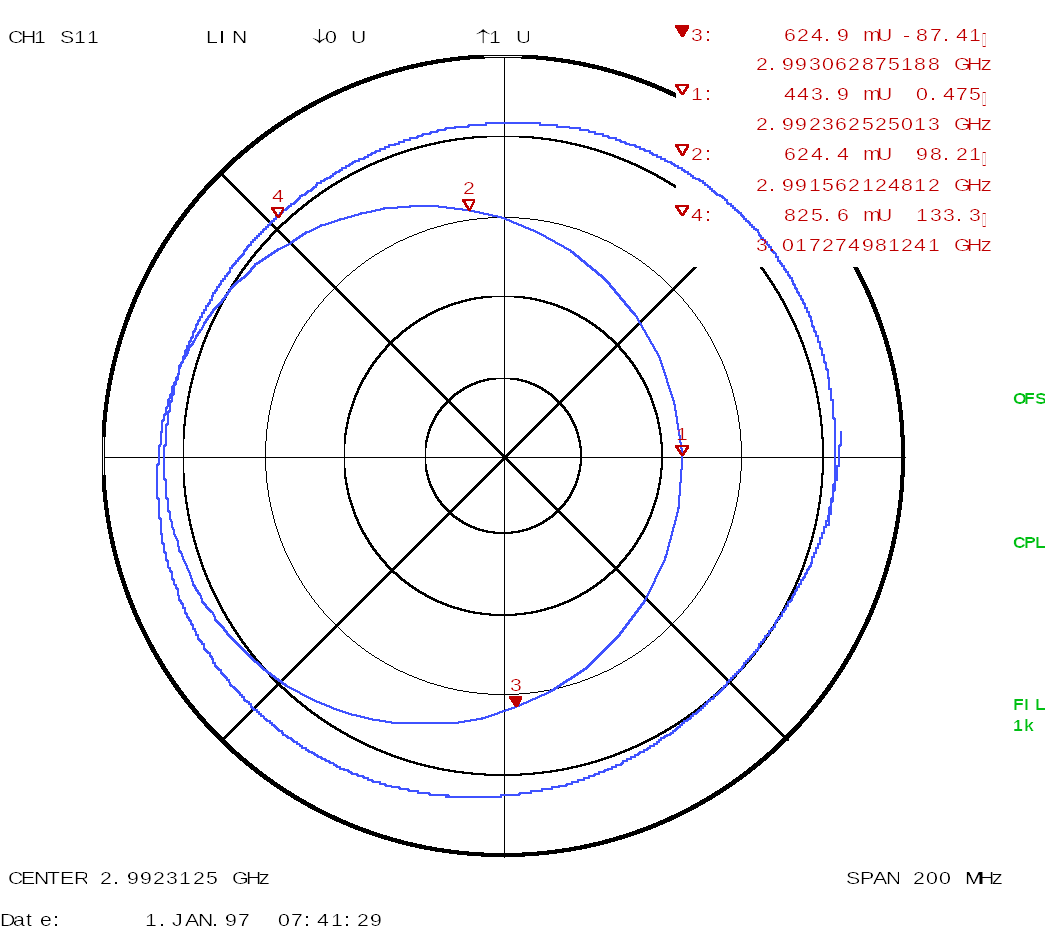
\includegraphics[width=0.7\columnwidth]{vectorial1.1.png}}}
	\quad
	\subfloat[Calibrated]{{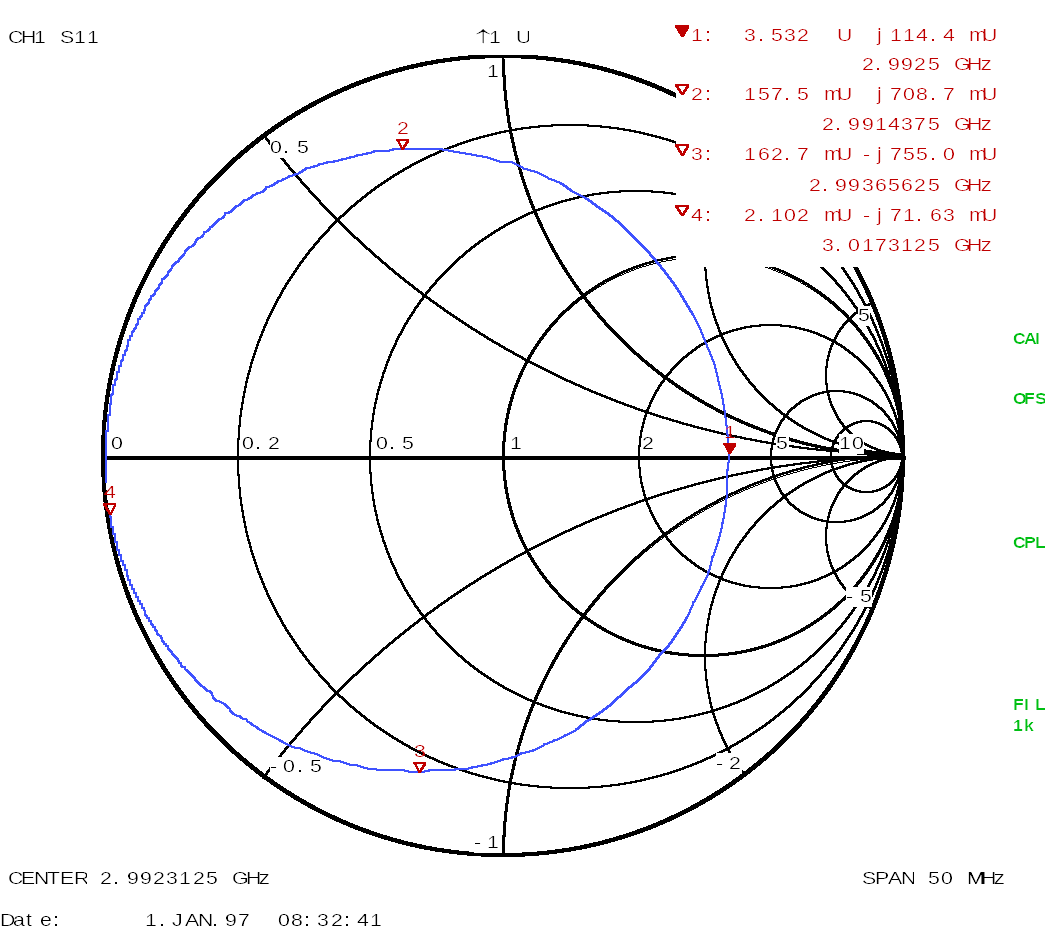
\includegraphics[width=0.7\columnwidth]{vectorial-smith.png}}}

	\caption{Vectorial measurement of the fundamental resonant mode (a) without
	and (b) with calibration. The curves are represented in linear polar and
	Smith representation respectively. The resonant frequency and points at
	half of the FWHM are indicated with markers 1, 2, 3 respectively.
	}
	\label{fig:vectorial_raw}
\end{figure*}

\subsection{Bead-Pull Measurement}
 

We then connected the coaxial cable to the cavity mounted on the rail. Using the
same method as with the scalar case, the location of the fundamental resonant
mode was determined and the resonant frequency and FWHM was tabulated. These
values were used to evaluate the quality factor $Q$, stored energy $W$, and the
power loss of the cavity. \par 

The cavity was then positioned such that the teflon bead was outside of the
cavity. The position of the cavity was then adjusted, and using the scalar
representation the change in resonant frequency $\Delta\omega_0$ and change in
reflection coefficient at resonant frequency $|\Delta\rho(\omega_0)|$ were
tabulated. The fluctuations and stepsize of the measurements were taken into
account as the uncertainties in measurement. This was performed until the bead
was completely outside of the cavity, which corresponds to a length of
approximately $\SI{40}{\milli\metre}$. The raw data can be observed in the
Appendix section. \par 

Using Eq. \ref{eqn:E0_res} and \ref{eqn:E0_nonres}, the unperturbed electric
field strength $E_0(z)$ was then determined for each position of the bead. Using
the power loss obtained from above, we then evaluated the shunt impedance $R_s$
as defined by Eq. \ref{eqn:Rs_res} and \ref{eqn:Rs_nonres} by
utilizing cubic interpolations and Gauss-Legendre quadrature integration
techniques. The transit time factor $\cos(\frac{\omega_0 z}{c})$ was also taken
into account when evaluating the shunt impedance, and the electric fields when
considering such time factor was compared to those without this factor. \par 

Finally, the energy gain of an accelerating particle $\delta U$ was determined for several
input powers using Eq. \ref{eqn:energy_gain}. This was used to observe if our cavity was suited for particle
accelerator experiments.

\chapter{Results and Discussion}

\section{Attenuation of Coaxial Cables}

Fig. \ref{fig:coax_atten} shows the attenuation of the RG142 and ST18 cables for frequency values at approximately 1, 2, 4,  and 7 $\si{\giga\hertz}$. 
The attenuations as given by the datasheets of the corresponding cable from the manufacturers are also shown \cite{st18,rg142}. To match the
amplitudes from our measurement with those from the datasheet, we had to apply a normalization factor of $N = \num{1e10}$ and $\num{1e2}$ for the 
RG142 and ST18 cables respectively. From the comparisons between the two attenuations, it is clear that the ST18 cable induces less power losses, 
even at higher frequencies. This implies that we should be using the ST18 cable for our measurement to prevent the signal loss in the coaxial
cable to influence our measurements. \par 

In our experiment, however, we have chosen to use the RG142 cable. This, as can be seen by Fig. \ref{fig:coax_atten}, will influence the reflection
measurements at higher frequencies. This may have been a main cause in the larger uncertainty in measurement of higher resonant modes. In the future,
the ST18 cable should be used instead of the RG142 cable. \par 

\begin{figure*}[htb!]
	\centering
	\subfloat[RG142
	]{{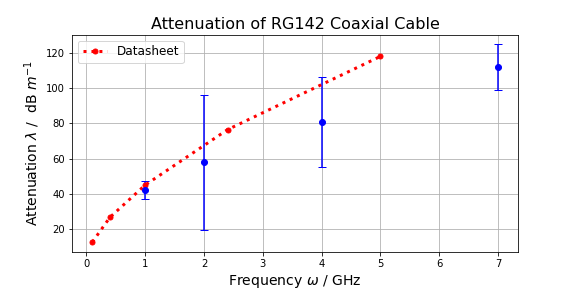
\includegraphics[width=0.48\columnwidth]{coax_atten_RG142.png}}}
	\quad
	\subfloat[ST18]{{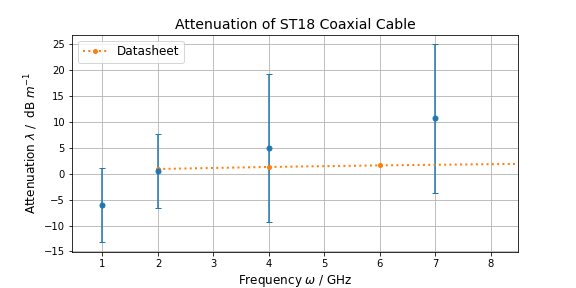
\includegraphics[width=0.48\columnwidth]{coax_atten_ST18.png}}}

	\caption{The attenuation of the (a) RG142 and (b) ST18 cable. }
	\label{fig:coax_atten}
\end{figure*}


\section{Scalar Measurement}

Tables \ref{tab:scalar_top} and \ref{tab:scalar_side} show the relevant parameters associated to each resonant mode in the cavity, i.e. the coupling coefficient $\kappa$, 
the FWHM $\Delta\omega_H$, the loaded and unloaded quality factor ($Q$, $Q_0$ respectively). The residual with the theoretical resonant frequency (table \ref{tab:mode_freq2})
 is also shown below. This is shown for the top and side cavity respectively. \par 

From our results, we observe that the resonant frequencies obtained are close to the theoretical values that we have computed analytically with a deviation of approximately 
$\sim 0.05 \si{\giga\hertz}$ for both cases. We observe that for all values of the coupling coefficient, they attain negative values, which is due to the fact that we have used 
dB as our unit of the reflection coefficient when calculating for $\kappa$ using Eq. \ref{eqn:kappa_rho}. This, however, had no notable effect on the measurement of the FWHM, as 
we attain reasonable values of the FWHM for both cases. \par 

When observing the loaded and unloaded quality factor, we see that values vary around $10^2 \sim 10^3$. In general, we observe that $Q > Q_0 / 2$, which implies
that most of the oscillatory modes that we obtain are undercritically coupled. The resonant mode with $\omega_0 = \SI{4.49725}{\giga\hertz}$, however, shown overcritical 
coupling instead, which yields a larger deviation from the theoretical resonant frequency. We also observe that as $Q \approx Q_0 / 2$, we obtain more accurate measurements
of the resonant frequency. \par  



\begin{table}[h!]
	\centering
	\begin{tabular}{|c|c|c|c|c|c|}
		\hline $\omega_0$/GHz & $\kappa$ & $\Delta\omega_H$/MHz & $Q (\cross 10^3) $ & $Q_0 (\cross 10^3)$ & $\left| \omega_0 - \omega_{thr} \right|$/GHz \\ 
		\hline 2.992206875 & $-1.4499 \pm 0.0010$  & 2.1375 & $1.3999 \pm 0.0093$ & $0.6298 \pm 0.0044$ & 0.0668\\ 
		\hline 4.53973125 &  $-1.0513 \pm 0.0066$ &  0.5750 & $7.90 \pm 0.19$ & $0.405 \pm 0.0053$ & 0.1214\\
		\hline 6.21559375 &  $ -2.460 \pm 0.053$  & 5.5625 & $1.1174 \pm 0.0028$ & $1.631 \pm 0.060$ & 0.0317\\
		\hline 6.940125 &  $-1.233 \pm 0.014$  & 5.6250 & $1.2338 \pm 0.0031$ & $0.288 \pm 0.017$ & 0.2251\\ 
		\hline 7.75975 &  $-1.639 \pm 0.016$  & 8.750 & $0.8868 \pm 0.0014$ & $0.556 \pm 0.014$ & 0.00153\\ 
		\hline
	\end{tabular}
	\caption{Calculated quantities for resonant modes for the top cavity. The residual with the analytical resonant frequency is also shown.}
	\label{tab:scalar_top}
\end{table}

\begin{table}[h!]
	\centering
	\begin{tabular}{|c|c|c|c|c|c|}
		\hline $\omega_0$/GHz & $\kappa$ & $\Delta\omega_H$/MHz & $Q (\cross 10^3)$ & $Q_0 (\cross 10^3)$ & $\left| \omega_0 - \omega_{thr} \right|$/GHz \\ 
		\hline 2.98690625 & $-2.4245 \pm 0.0051$ & 4.0625 & $0.7352 \pm 0.0026$ & $1.0473 \pm 0.0052$ & 0.0615 \\ 
		\hline 4.49725 & $-8.41 \pm 0.55$ & 1.375 & $3.270 \pm 0.034$ & $242 \pm 18$ & 0.1640 \\
		\hline 6.2078875  & $ -1.7270 \pm 0.0026$ & 0.8125 & $7.64 \pm 0.13$ & $5.555 \pm 0.099$ & 0.0394 \\
		\hline 7.74540625  & $-1.3556 \pm 0.0019$ & 0.875 & $8.85 \pm 0.14$ & $3.147 \pm 0.054$ & 0.0158 \\ 
		\hline
	\end{tabular}
	
	\caption{Same as Table \ref{tab:scalar_top} but for the side cavity. }
	\label{tab:scalar_side}
\end{table}

We now compare between the results of the top and side cavity. We first notice that while we were able to observe 5 resonant modes in the top cavity, only 4 such modes
were observed in the side cavity. This may be caused by the longitudinal-dependence of the missing resonant mode (corresponding to the $TM_{020}$), as the side coupling
may have affected the signal going through the cavity. Fig. \ref{fig:scalar_residual} shows the difference between the resonant frequencies obtain from the top and side cavity.
From this, we observe that deviations are on order $10^{-2}$, yielding similar results between the two couplings. We further observe that for the resonant mode at 
$\omega \approx \SI{4.49}{\giga\hertz}$, the deviation is the largest. This may be caused by the overcritical coupling observed from the side cavity at this resonant frequency
as mentioned previously.\par 


\begin{figure*}[h!]
	\centering
	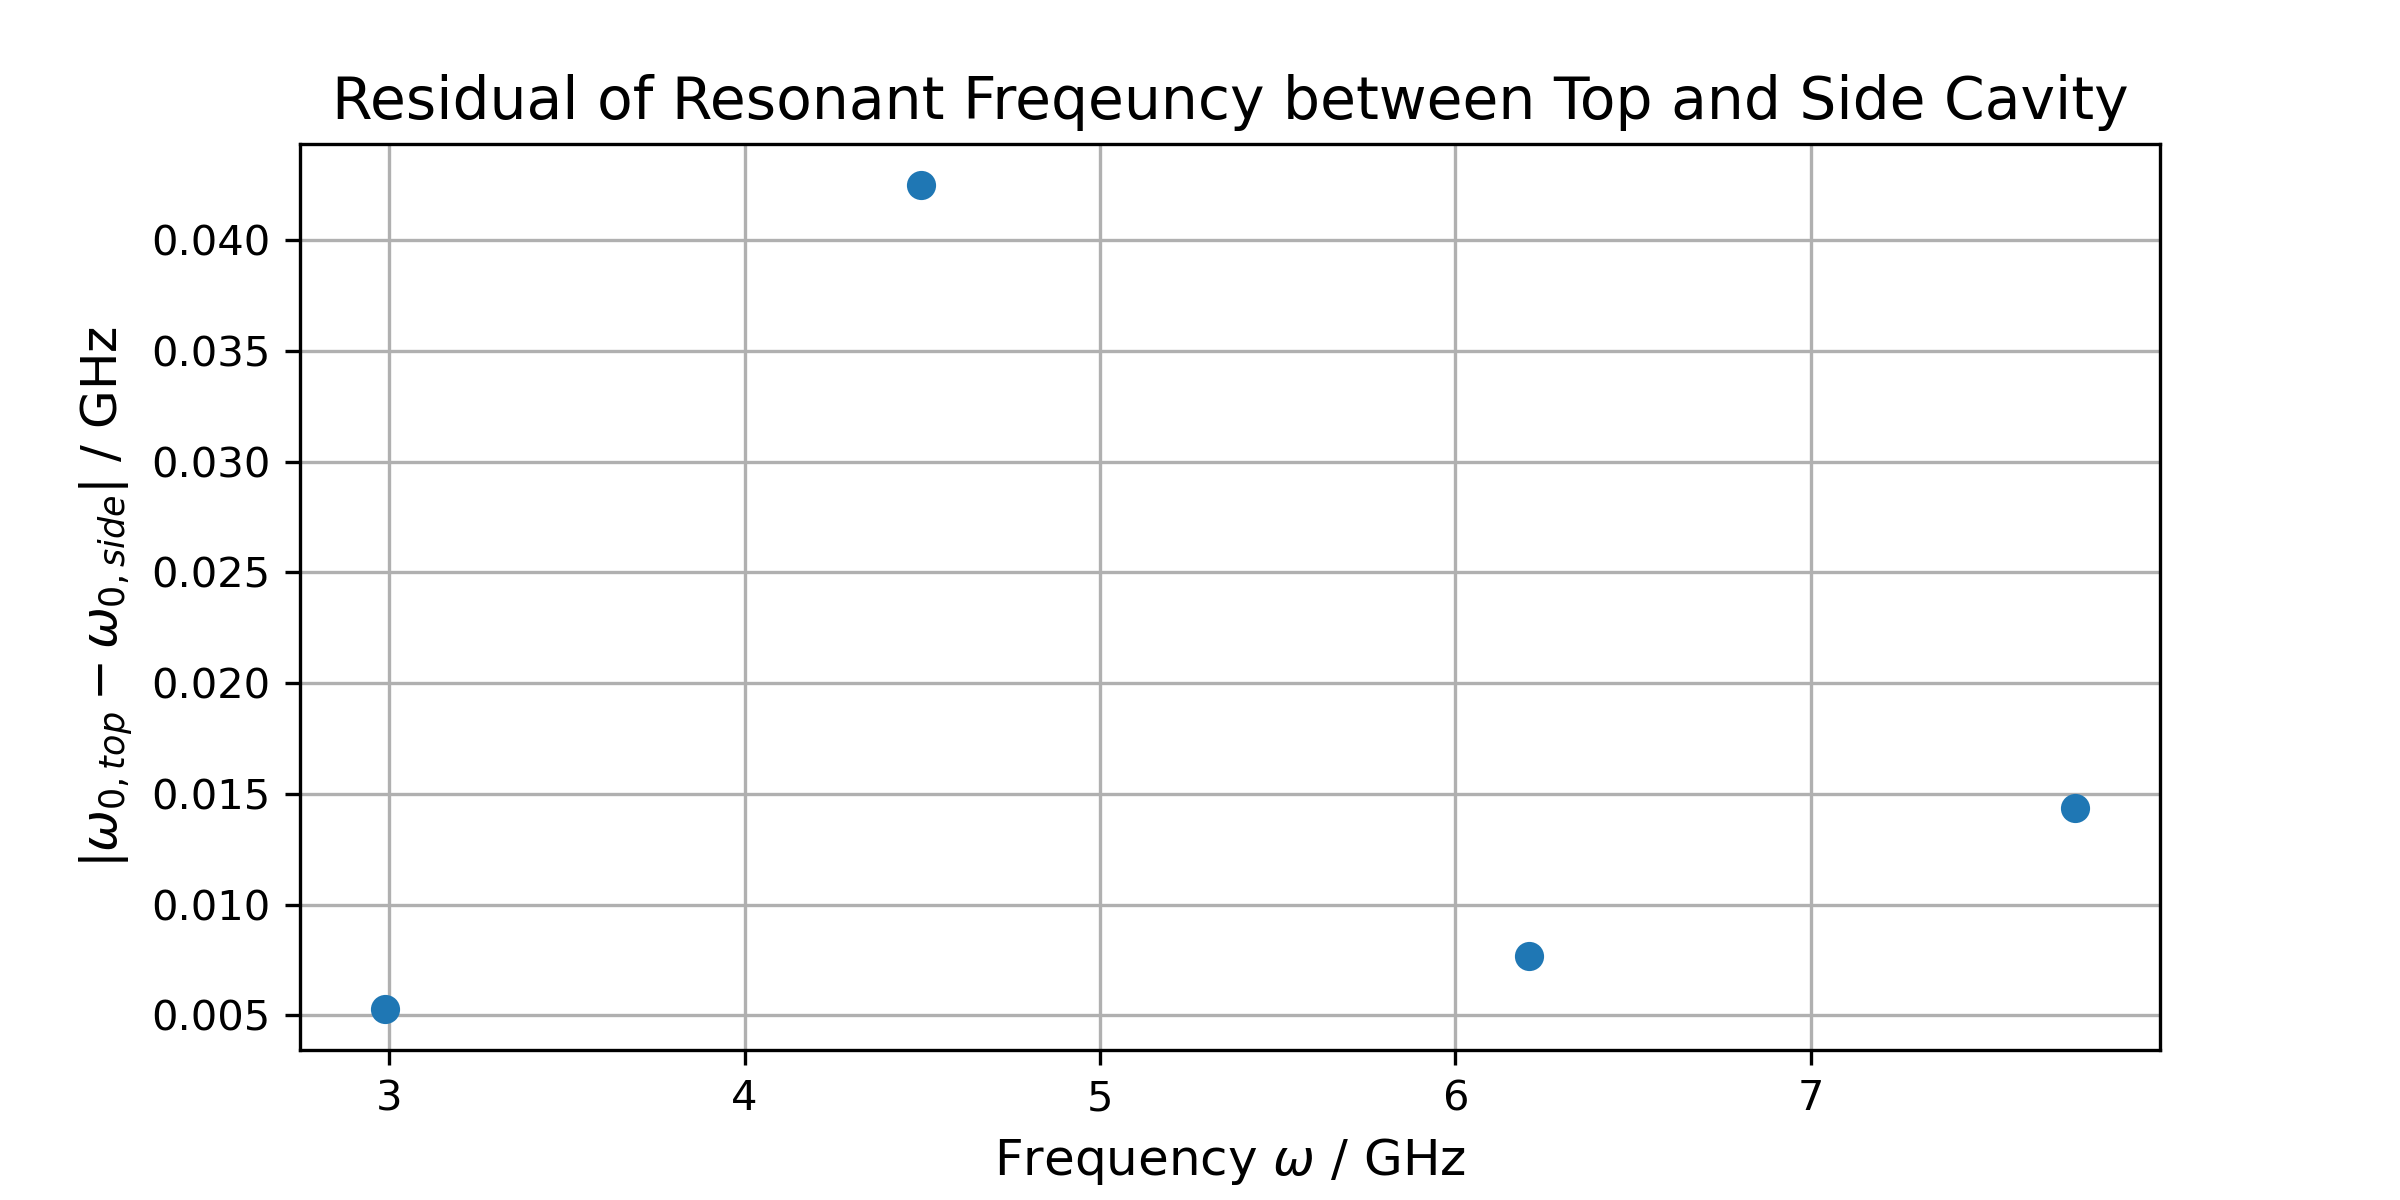
\includegraphics[width=0.6\columnwidth]{scalar_residual_topside.png}
	\caption{Residual between the resonance frequencies of the top and side cavity. }

	\label{fig:scalar_residual}
\end{figure*}

\section{Vectorial Measurement}

Table \ref{tab:vectorial} shows the measured and calculated quantities obtained from the vectorial measurement at the fundamental resonant mode. This is 
shown both for the uncalibrated and calibrated measurements. Between the two measurements, we observe that the quality factor from the calibrated results
is much larger, indicating a better measurement after calibration. The power lost between the two measurements do not differ, implying that the calibration
does not largely affect the power lost in the system. \par 

\begin{table}[h!]
	\centering
	\begin{tabular}{|c|c|c|}
		\hline  & Uncalibrated & Calibrated \\ 
		\hline $\omega_0$ / GHz & 2.992362525013 & 2.9915625 \\
		\hline $\kappa$ & $-1.0045157 \pm 0.0000051$ & $-1.0049865\pm 0.0000030$ \\
		\hline $\Delta\omega_H$ / MHz & 3.001 & 2.219 \\
		\hline $Q_0$  & $1998.407 \pm 0.012$  & $3368.1 \pm 2.1$  \\
		\hline $Q_{ext}$ & $1989.435 \pm 0.015$ & $2248.3 \pm 1.4$ \\
		\hline SWR $S$ & $1.0045157 \pm 0.0000051$ & $1.003447 \pm 0.0000030$ \\
		\hline $P$ / mW & $1.567 \pm 0.023$ & $1.567 \pm 0.023$\\ 
		\hline   
	\end{tabular}
	\caption{Calculated quantities from uncalibrated and calibrated vectorial measurement. }
	\label{tab:vectorial}
\end{table}

Comparing our obtained data to those from the scalar measurement in Table \ref{tab:scalar_top}, we observe that the quality factor obtained is much larger, and the value of $\kappa$ is more
closer to unity, indicating that with this measurement, the accuracy of the experiment increases. This is also observed by the standing wave ratio, as its value is close to unity. This tells
us that the vectorial method yields a more accurate and stable result. \par

% In this experiment, we were not able to realize the proper measurement method as instructed, and a direct conversion of the scalar to the vectorial representation was performed instead.
% In this sense, it is relatively hard to compare the properties between the two results. 


% \begin{table}[h!]
% 	\centering
% 	\begin{tabular}{|c|c|c|c|c|c|c|}
% 		\hline Type & $\kappa$ & $\Delta\omega_H$ / MHz & $Q_0$ & $Q_{ext}$ & $S$ & $P$ / mW\\ 
% 		\hline Uncalibrated & $-1.0045157 \pm 0.0000051$ & 3.001 & $1998.407 \pm 0.012$ 
% 				& $1989.435 \pm 0.015$ & $1.0045157 \pm 0.0000051$ & $1.567 \pm 0.023$\\ 
% 		\hline Calibrated & $-1.0049865\pm 0.0000030$ & 2.219 & $3368.1 \pm 2.1$ 
% 				& $2248.3 \pm 1.4$ & $1.003447 \pm 0.0000030$ & $1.567 \pm 0.023$\\
% 		\hline
% 	\end{tabular}
% 	\caption{Calculated quantities from uncalibrated and calibrated vectorial measurement. }
% 	\label{tab:vectorial}
% \end{table}

\section{Bead-Pull Measurement}

From the bead-pull measurement, we first determined the relevant quantities at the fundamental resonant mode, corresponding to 
the TEM$_{010}$ mode. Table \ref{tab:bead_pull} shows the parameters obtained from our measurement with an input power of $P_0 = 1.189 \pm 0.01151$ mW.
All values were calculated as with the previous section, and the stored energy $W = Q_0 P / \omega_0$. \par 


\begin{table}[h!]
	\centering
	\begin{tabular}{|c|c|c|c|c|c|}
		\hline $\omega_0$ / GHz & $\kappa$ & $\Delta\omega_H$ / MHz & $Q$ & $P$ / mW & $W$ / nJ\\ 
		\hline $2.9939375$ & $1.197230 \pm 0.000058$ & 0.712 & $4205 \pm 42$ 
				& $1.1789 \pm 0.0114$ & $ 3.638 \pm 0.050$ \\ \hline
	\end{tabular}
	\caption{Calculated quantities for scalar measurement with the mounted cavity, used for the bead-pull measurement.}
	\label{tab:bead_pull}
\end{table}

We then evaluated for the electric field $E_0$ using both resonant and non-resonant methods. Fig. \ref{fig:E0} shows the 
electric field as a function of the position of the bead $z$ with and without including the time transit factor $\cos(\omega_0 z / c)$. \par 

\begin{figure*}[htb!]
	\centering
	\subfloat[Without time transit factor]{{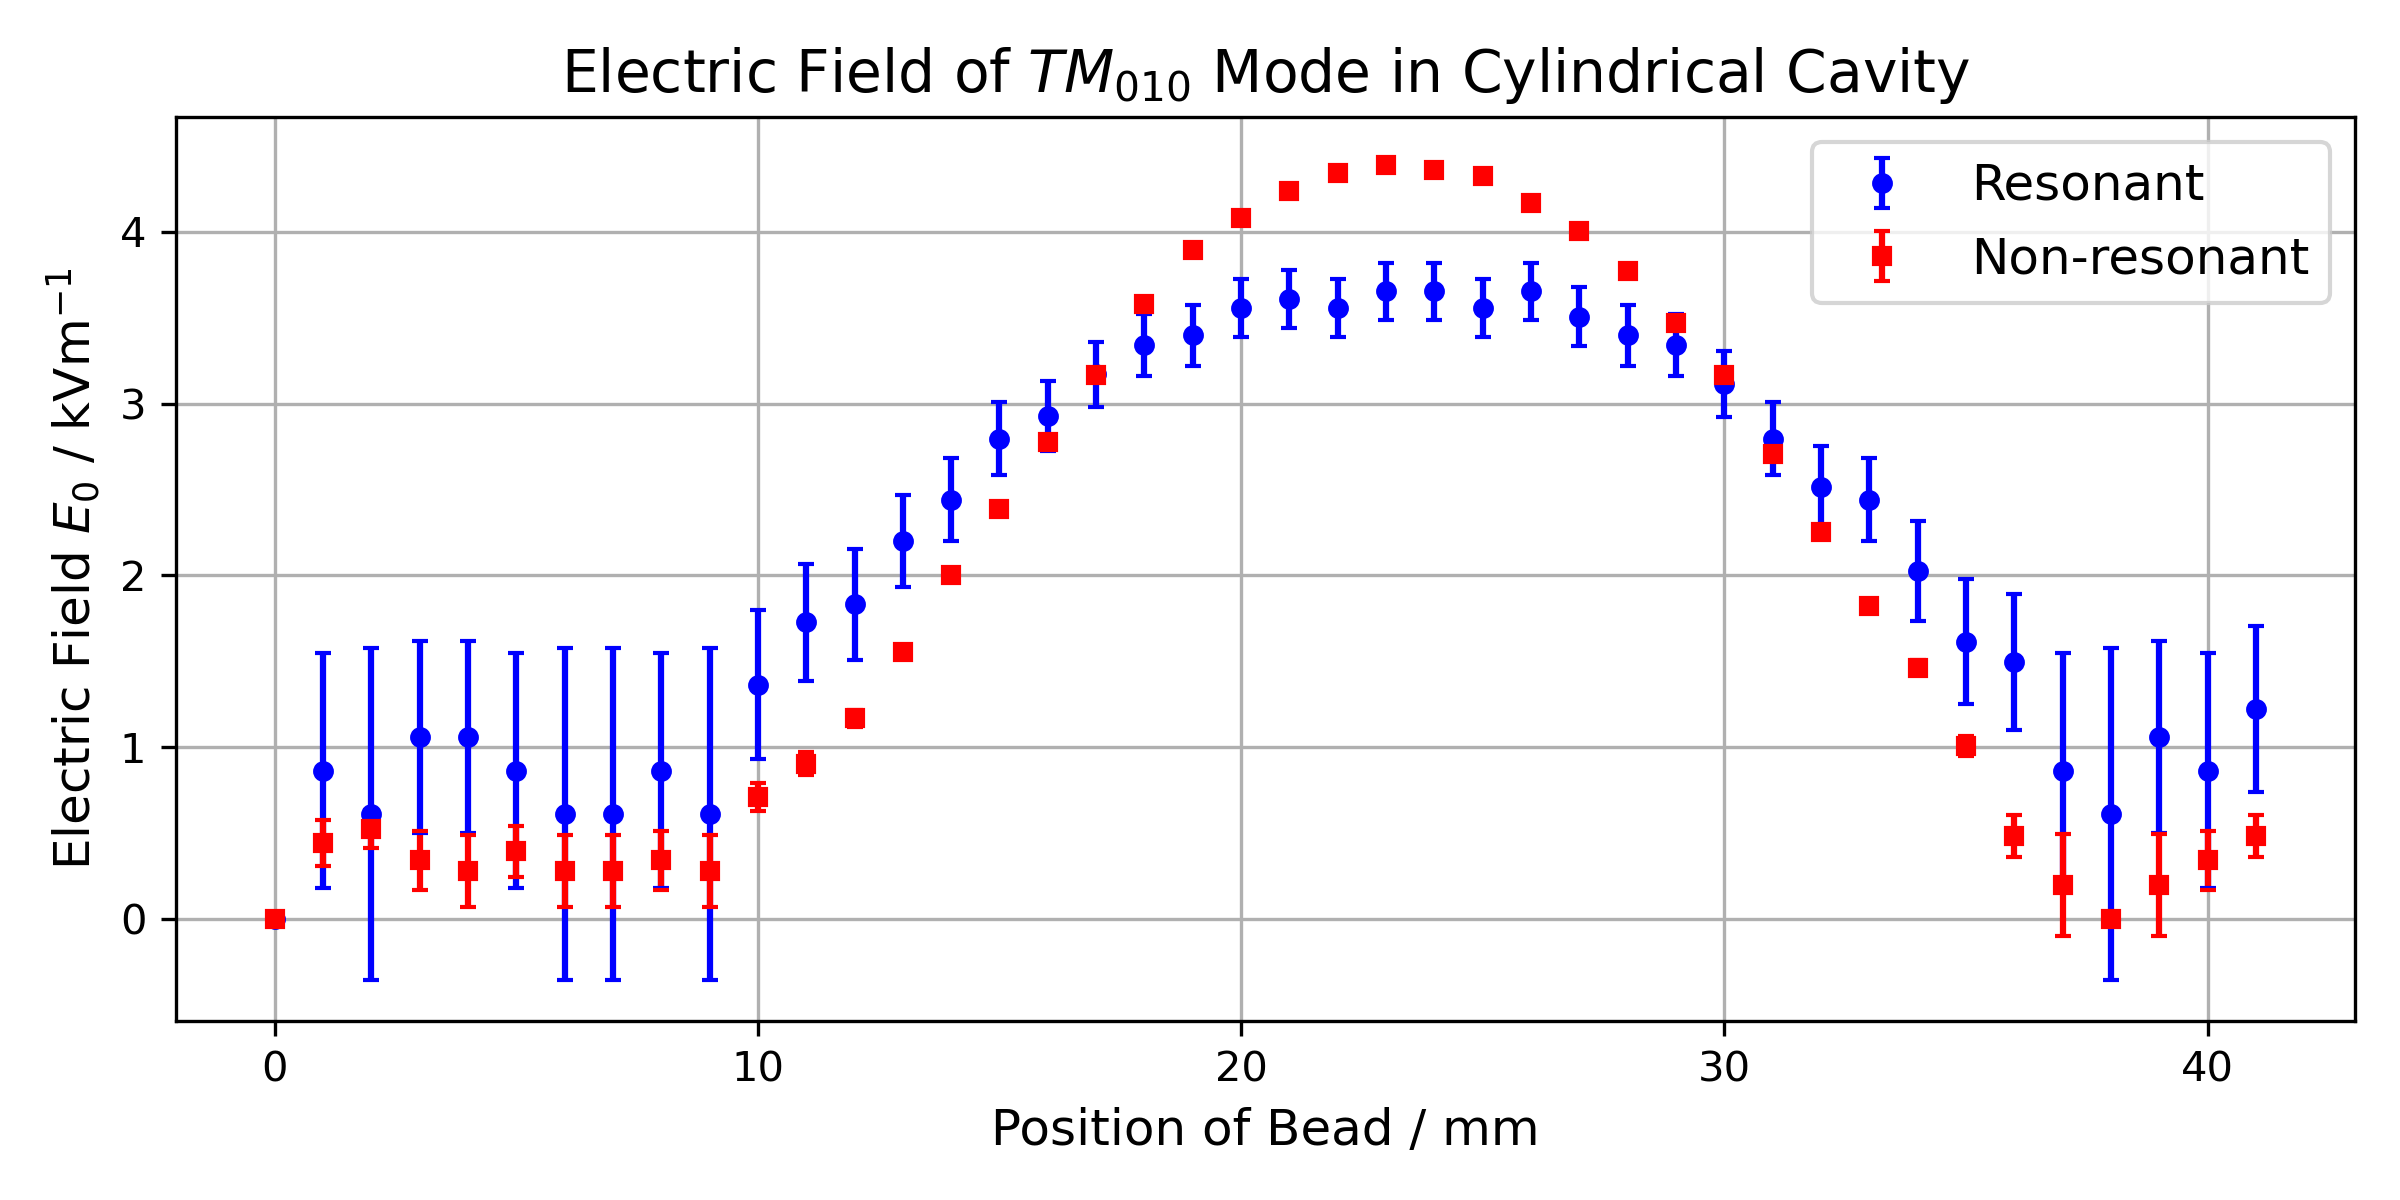
\includegraphics[width=0.48\columnwidth]{E0_nott.png}}}
	\quad
	\subfloat[With time transit factor]{{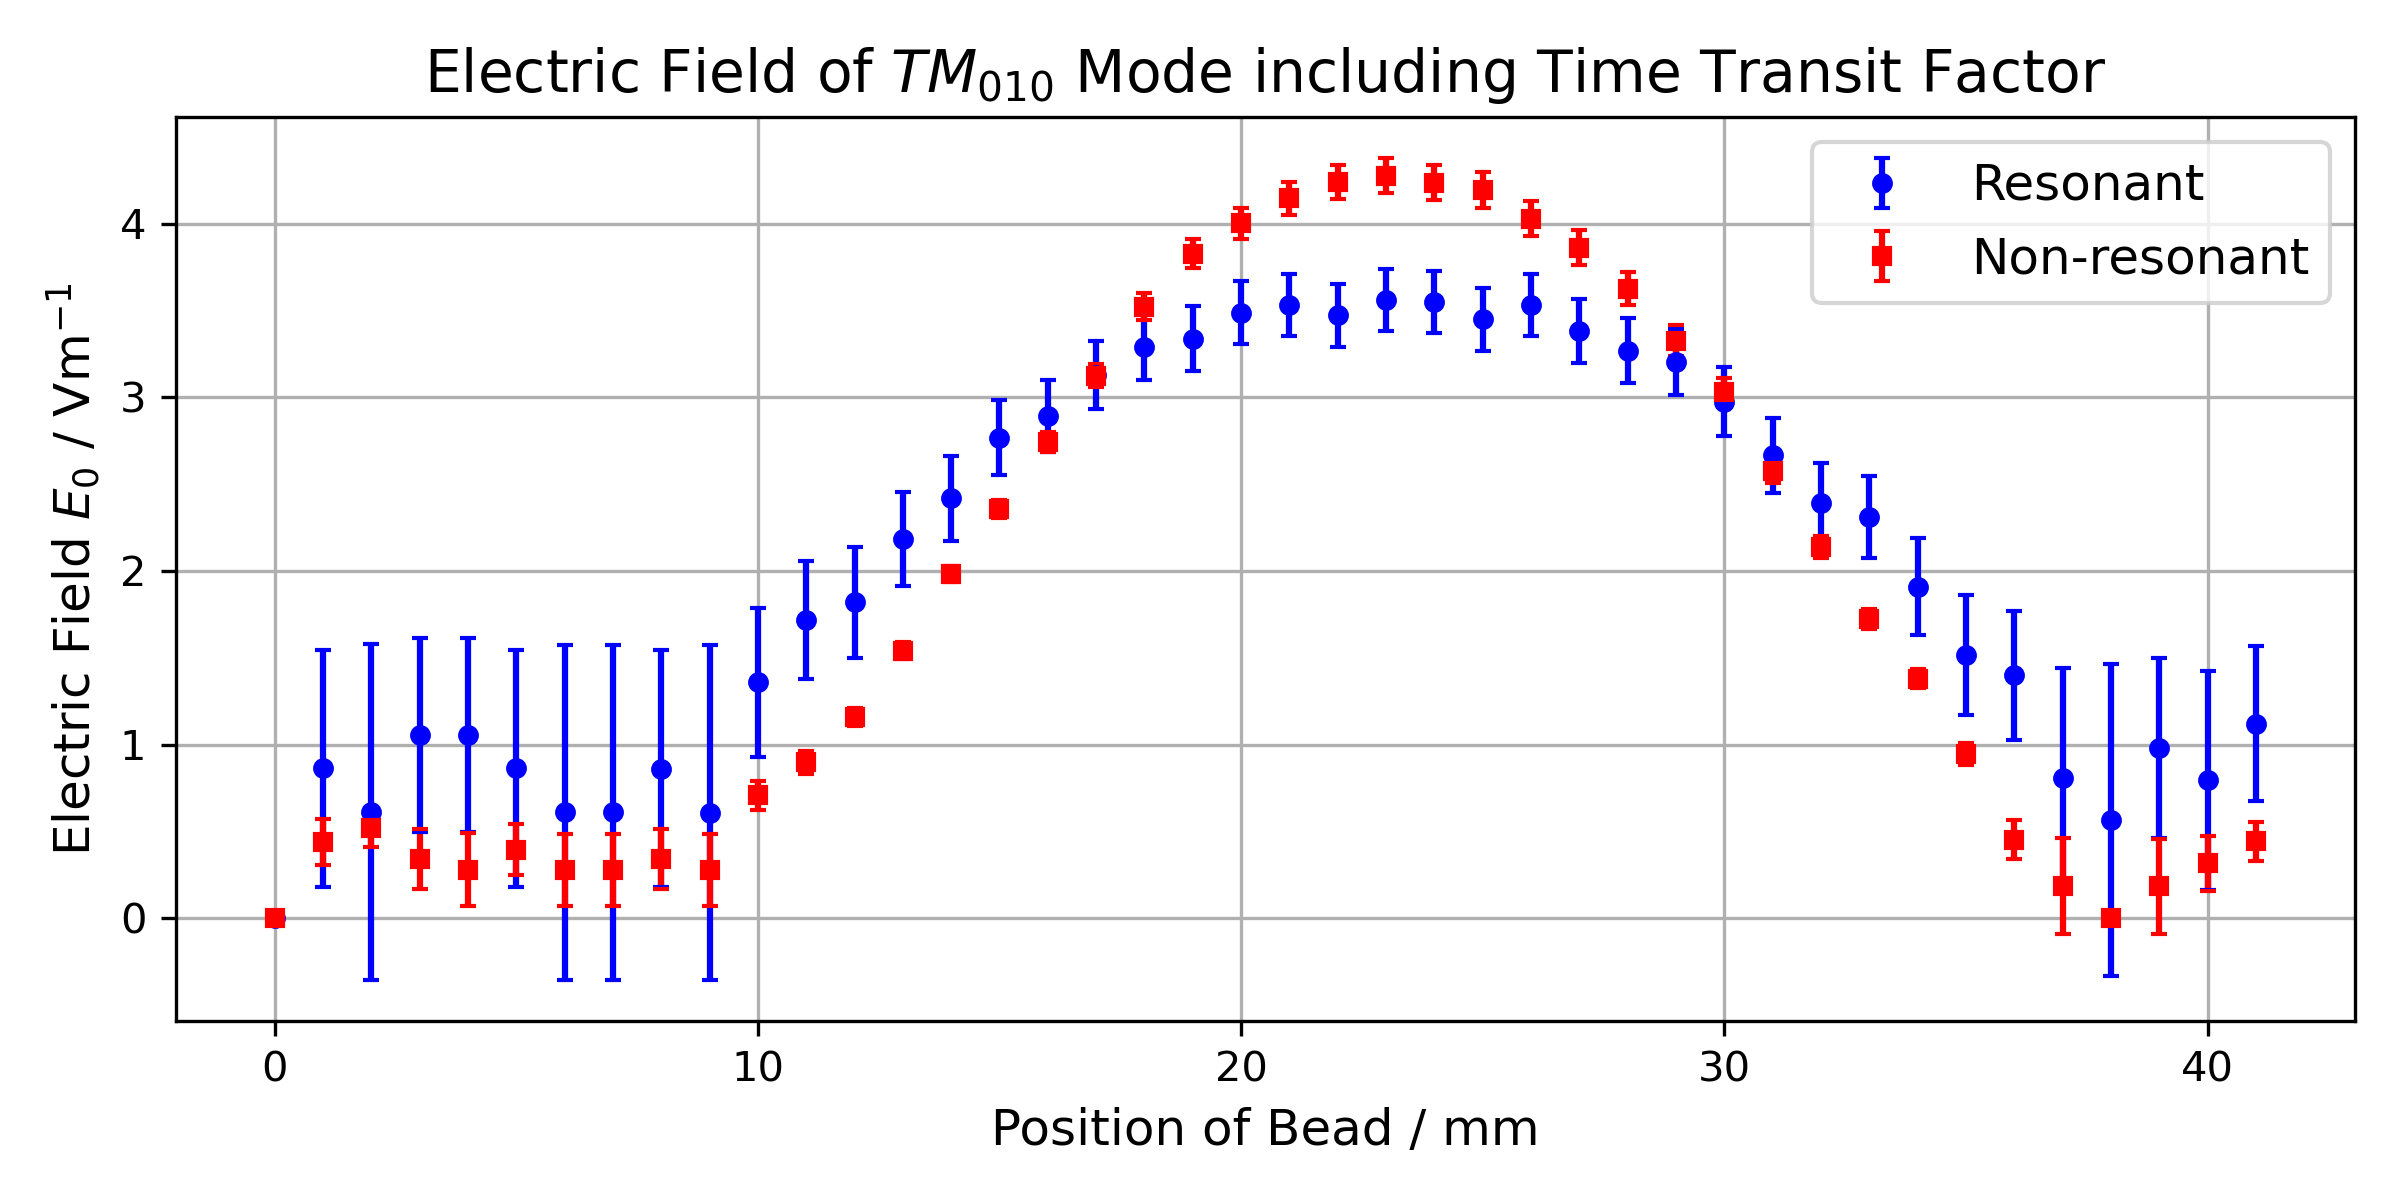
\includegraphics[width=0.48\columnwidth]{E0_tt.png}}}

	\caption{The electric field $E_0$ for different positions of the bead $z$ (a) not including and 
			(b) including the time transit factor. The results from both resonant and non-resonant method are shown.}
	\label{fig:E0}
\end{figure*}

We observe that while both behaviours yield similar oscillatory behaviours, the results from the resonant method have a 
flatter curve with a lower maximal amplitude of $\SI{3.65 \pm 0.16}{\kilo\volt\per\metre}$ compared to the non-resonant method, which has
a maximal amplitude of $\SI{4.390 \pm 0.040}{\kilo\volt\per\metre}$. Furthermore, the uncertainty of the results from the resonant
method also have larger uncertainties compared to the non-resonant method. As both measurements should ideally yield the same result,
such difference between the two methods may have been caused by imperfect calibrations before measurement. When we include the time transit factor,
 we observe that the amplitude of the electric field decreases, yielding a maximal amplitude of  $\SI{3.56 \pm 0.18}{\kilo\volt\per\metre}$
 and $\SI{4.27 +- 0.10}{\kilo\volt\per\metre}$ for the resonant and non-resonant method respectively. The overall structure, however,
 does not differ with the inclusion of this factor.\par 

We now evaluate the shunt impedance using the obtained electric field and the corresponding parameters determined from Table \ref{tab:vectorial}.
This was performed for the results obtained from both the resonant and non-resonant method using Eq. \ref{eqn:Rs_nonres} and \ref{eqn:Rs_res}.
After performing integration, we obtain the following for the shunt impedance:
\begin{align*}
	R_{s, res} = \SI{3.316 \pm 0.032}{\mega\ohm} \\
	R_{s, non\text{-}res} = \SI{3.791 \pm 0.037}{\mega\ohm}
\end{align*}

Using the shunt impedence we obtained for our cavity, we can determine if our cavity is sufficient to accelerate particles. To do this,
we first calculate the energy gain of a particle (here, an electron) after passing through our cavity with different input powers.
Table \ref{tab:energy_gain} show the energy gain using the shunt impedance evaluated from both resonant and non-resonant methods for 
different input radiofrequency powers $P_0$.

\begin{table}[h!]
	\centering
	\begin{tabular}{|c|c|c|}
		\hline $P_0$ / kW & $\delta U_{res}$ / keV & $\delta U_{non\text{-}res}$ / keV \\
		\hline 1 & $56.52 \pm 0.27$ & $60.43 \pm 0.29$ \\ 
		\hline 10 & $178.72 \pm 0.86$ & $191.10 \pm 0.93$ \\ 
		\hline 100 & $565.2 \pm 2.7$ & $604.3 \pm 2.9$ \\ 
		\hline 1000 & $1787.2 \pm 8.7$ & $1910.1 \pm 9.3$ \\ 
		\hline
	\end{tabular}
	\caption{Energy gain of electron under cavity used in this experiment for several input radiofrequency powers.}
	\label{tab:energy_gain}
\end{table}

We observe that for an input power of $\SI{100}{\kilo\watt}$, we obtain an energy gain on the order of $\SI{100}{\kilo\electronvolt}$, 
which is a factor of 10 lower than typical values for acceleration energies for particles with this input power. This 
shows that our cavity is not suitable to accelerate particles. \par 

\chapter{Conclusion and Outlook}

\section{Conclusion}

In our experiment, we observed if a given cavity was suitable for particle acceleration. To this end, we had to first determine
the reflection coefficient of the signal transmitted through the coaxial cable at different resonant modes of the cavity. This
would yield reflection curves that dip sharply to $|\rho| \approx 0$ near resonance of the cavity. In order to determine the 
most efficient coaxial cable to use (i.e. that with the least power loss), the attenuation of the coaxial cable was measured. 
While we observed that the ST18 coaxial cable yield lower attenuation, we used the RG142 cable instead. In future experiments,
the attenuation of the cable should be carefully considered before performing the rest of the measurements. \par 

The resonant frequencies at dips in the reflection curve was measured using a Vector Network Analyzer (VNA), and from this the coupling coefficient $\kappa$
and $|\rho(\Delta\omega_H / 2)|$ was computed. The FWHM of the curve was then measured from such values. The quality factor $Q$, 
which quantifies the degree of damping in the system, was then computed. In our analysis, we compared the behaviour between\par 
avities which differed in their location of coupling which yielded deviations of order $10^{-2}$. Deviations between the 
analytical resonant frequencies were also as large as $10^{-2}$, which indicate that our results are in good agreement with
expected values. The relationship between the quality factor and the comparison with theoretical values were also observed. \par 

The results from the scalar measurement was also compared from those obtained by measuring the corresponding values in a vectorial representation. In this way, the corresponding quantities are much easier to 
obtain as the coupling coefficient, resonant frequency, and FWHM can be determined pictorially using a Smith diagram. We, however,
used the same scalar method to measure the resonant frequency and observed the corresponding data in a vectorial representation. 
In future experiments, proper measurements in this format should be performed. \par 

To directly quantify the performance of acceleration for charged particles, we performed a bead-pull measurement where the 
perturbation of the resonant frequency and $|\rho(\omega_0)$ was measured due to a bead passing through the cavity. The 
electric field within the cavity was computed using two different methods which showed similar structures with different 
maximal amplitudes. After taking into account of the time transit factor, the shunt impedance was evaluated, yielding
$R_{s, res} = \SI{3.316 \pm 0.032}{\mega\ohm}$ and $R_{s, non\text{-}res} = \SI{3.791 \pm 0.037}{\mega\ohm}$ for the 
resonant and non-resonant method respectively. These impedances were used to quantify the energy gain of an electron in our cavity
at different input powers. This did not yield sufficient acceleration voltages for the electron, implying that our cavity is not
suited for particle acceleration. \par 

\section{Outlook}

This experiment consisted of a lot of small details that needed to be taken into account. Due to the time constraints, it is 
vital to be able to operate the VNA smoothly. This will yield less uncertainty and confusion when performing measurements. 
Furthermore, each step should be carefully verified and comprehended (as with the attenuation of the coaxial cable) before
moving to the next step, as small misconceptions may allow measurements that are not as accurate as one could have done. 
To extend such an experiment, one can observe the resonant frequencies for different cavity geometries. This can also be done 
by considering cavities with different materials, ex copper vs iron. 


\chapter{Appendix}

In this section, we will provide with supplementary data that is not within the scope of the main report, but can nevertheless
be useful to observe. 

\begin{table}[!ht]
    \centering
    \begin{tabular}{|c|c|c|}
    \hline
        $z$ / mm & $\Delta\omega_0$ / kHz & $|\Delta\rho|$ / dB \\ \hline
        41.1 & 0 & 0 \\ \hline
        42.1 & 6.25 & 0.005 \\ \hline
        43.1 & 3.125 & 0.007 \\ \hline
        44.1 & 9.375 & 0.003 \\ \hline
        45.1 & 9.375 & 0.002 \\ \hline
        46.1 & 6.25 & 0.004 \\ \hline
        47.1 & 3.125 & 0.002 \\ \hline
        48.1 & 3.125 & 0.002 \\ \hline
        49.1 & 6.25 & 0.003 \\ \hline
        50.1 & 3.125 & 0.002 \\ \hline
        51.1 & 15.625 & 0.013 \\ \hline
        52.1 & 25 & 0.021 \\ \hline
        53.1 & 28.125 & 0.035 \\ \hline
        54.1 & 40.625 & 0.062 \\ \hline
        55.1 & 50 & 0.103 \\ \hline
        56.1 & 65.625 & 0.146 \\ \hline
        57.1 & 71.875 & 0.198 \\ \hline
        58.1 & 84.375 & 0.258 \\ \hline
        59.1 & 93.75 & 0.329 \\ \hline
        60.1 & 96.875 & 0.390 \\ \hline
        61.1 & 106.2 & 0.428 \\ \hline
        62.1 & 109.37 & 0.461 \\ \hline
        63.1 & 106.2 & 0.484 \\ \hline
        64.1 & 112 & 0.495 \\ \hline
        65.1 & 112 & 0.488 \\ \hline
        66.1 & 106.2 & 0.481 \\ \hline
        67.1 & 112 & 0.446 \\ \hline
        68.1 & 103.12 & 0.412 \\ \hline
        69.1 & 96.875 & 0.365 \\ \hline
        70.1 & 93.75 & 0.309 \\ \hline
        71.1 & 81.25 & 0.258 \\ \hline
        72.1 & 65.625 & 0.188 \\ \hline
        73.1 & 53.125 & 0.130 \\ \hline
        74.1 & 50 & 0.085 \\ \hline
        75.1 & 34.375 & 0.055 \\ \hline
        76.1 & 21.875 & 0.026 \\ \hline
        77.1 & 18.75 & 0.006 \\ \hline
        78.1 & 6.25 & 0.001 \\ \hline
        79.1 & 3.125 & 0 \\ \hline
        80.1 & 9.375 & 0.001 \\ \hline
        81.1 & 6.25 & 0.003 \\ \hline
        82.1 & 12.5 & 0.006 \\ \hline
    \end{tabular}
	\caption{$\Delta\omega_0$ and $|\Delta \rho|$ from the bead-pull measurement at different positions of the bead.}
\end{table}

\printbibliography

\end{document}
